\documentclass[a4paper,english]{report}
\usepackage[utf8]{inputenc}
\setcounter{secnumdepth}{3}
\usepackage{babel}
\usepackage{array}
%\usepackage{booktabs}
\usepackage{textcomp}
\usepackage{url}
\usepackage{multirow}
\usepackage{amsmath}
\usepackage[section]{placeins}
\usepackage{gensymb}
\usepackage{graphicx}
\usepackage[authoryear]{natbib}
\usepackage{nomencl}
\providecommand{\printnomenclature}{\printglossary}
\providecommand{\makenomenclature}{\makeglossary}
\makenomenclature
\usepackage[unicode=true,
 bookmarks=false,
 breaklinks=false,pdfborder={0 0 1},backref=section,colorlinks=false]
 {hyperref}
\usepackage{breakurl}
\usepackage{etoolbox}
\makeatletter
\patchcmd{\Ginclude@eps}{"#1"}{#1}{}{}
\makeatother

%\makeatletter
%\special{papersize=\the\paperwidth,\the\paperheight}

%\newcommand{\noun}[1]{\textsc{#1}}
%\providecommand{\tabularnewline}{\\}
%\newcommand{\lyxdot}{.}


\usepackage[colorinlistoftodos]{todonotes}
%\usepackage{placeins}
%\usepackage{parskip}



\usepackage{subcaption}
\usepackage{tikz}

\usepackage{array}

\usepackage{amssymb}


\usepackage{graphicx}

%\usepackage{booktabs}
%\newcommand{\otoprule}{\midrule[\heavyrulewidth]}

%\usepackage{pdflscape}
%\usepackage{bbding}
%\usepackage{pifont}

\makeatother

\begin{document}
\thispagestyle{empty}

\vspace*{3cm}

\begin{center}
{\LARGE{}Marine Cybernetics}
\par\end{center}{\LARGE \par}

\begin{center}
{\LARGE{}Laboratory Handbook }
\par\end{center}{\LARGE \par}

\begin{flushleft}
\vfill{}
\par\end{flushleft}

\begin{flushleft}

\includegraphics[scale=0.6]{fig/NTNU_logo.pdf}
\par\end{flushleft}

Faculty of Engineering Science and Technology\\
Department of Marine Technology

\clearpage{}\thispagestyle{empty}\vspace*{3cm}
\begin{table}[h!]
	\centering
	\caption*{\huge{\textbf{Device network addresses}}}
	\begin{tabular}{lll}
		\hline
		\textbf{Qualisys PC} & 192.168.0.10 & surface\\
		& 192.168.0.20 & underwater\\ \hline
		\textbf{MCLab router} & 192.168.0.50 & SSID: MC Lab\\ \hline
		\textbf{RPi} & 192.168.1.22:51717 & for all\\ \hline
		\textbf{cRIO primary port} & 192.168.0.71 & IIMT-HILLAB1-cRIO\\
		& 192.168.0.72 & IIMT-HILLAB2-cRIO\\
		& 192.168.0.73 & IIMT-HILLAB3-cRIO\\
		& 192.168.0.75 & CSE1-cRIO\\
		& 192.168.0.55 & CSAD-cRIO\\
		\textbf{cRIO secondary port} & 192.168.1.21 & for all\\ \hline
		\textbf{Assigned by DHCP} & From 192.168.0.100 & \\
		& to 192.168.0.254 & \\ \hline
		\textbf{Subnet mask} & 255.255.255.0 & for all\\ \hline
	\end{tabular}
\end{table}
\clearpage{}

\pagenumbering{roman}\setcounter{page}{1}

\vspace*{3cm}

\section*{Introduction}

This handbook is Version 2.0 of the Marine Cybernetics Laboratory Handbook. The handbook gives a description of the equipment in the MCLab, and instructions on some of the software used. Every student using the MCLab should read this document before using equipment in the lab. In addition to this Handbook, there are separate handbooks for CS Enterprise 1 and CS Arctic Drill Ship, which are found on GitHub. As of July 2017, the other vessels do not have a separate Handbook, and thus the reader is referred to the old MCLab Handbook for complementary information about the specific vessel. 

\section*{Structure}
Chapter \ref{ch:marine_cybernetics_laboratory_equipment} describes the different equipment found in the Laboratory, and how to use it. \\
\noindent
Chapter \ref{ch:software} gives a description of some of the software used in the lab. This includes formatting and installing software on cRIO, creating FPGA modules, mapping of channels in VeriStand etc. 

\newpage{}
\tableofcontents{}
\clearpage
\pagenumbering{arabic}
\chapter{Marine Cybernetics Laboratory equipment}\label{ch:marine_cybernetics_laboratory_equipment}
\section{Introduction}
The laboratory is equipped for experimental testing of marine control systems and hydrodynamic tests. It consists of a wave basin with an advanced instrumentation package and a towing carriage. The basin, depicted in Figure \ref{fig: Marine cybernetics laboratory basin-1}, has dimensions 40m x 6.45m x 1.5m (LxBxD). The laboratory consists of the following fixed equipment: 
\begin{itemize}
	\item Qualisys Motion Capture System
	\item Towing Carriage
	\item Wave Generator
	\item Video-camera
\end{itemize}
These parts are thouroghly described in the next sections, with a user manual and technical description of the equipment. 

\begin{figure}[h!]
	\centering 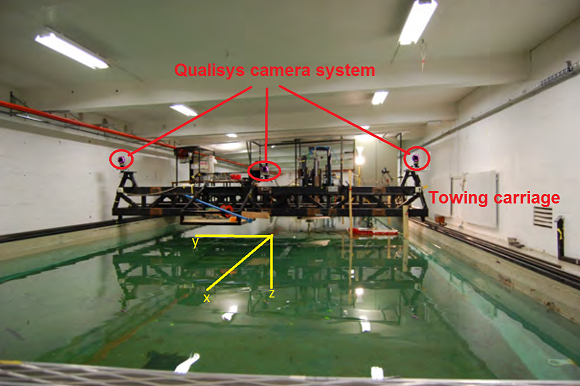
\includegraphics[width=0.95\textwidth]{fig/mc_lab} 
	\caption{Marine cybernetics laboratory basin}
	\label{fig: Marine cybernetics laboratory basin-1}
\end{figure}

\subsection{Safety}\
\subsubsection{Personnel injury}
\paragraph{Drowning}
It is required to have two or more persons present when using the basin.
\paragraph{Electric shock}
The towing catenary should not be approached or touched.
\paragraph{Carriage collision}
It is forbidden to run the towing carriage when there are people alongside the basin.
\paragraph{Thruster blade cuts}
Vessels must stay in the water as long as actuators are active. Before removing the vessels from the water, the control system must be stopped and disabled, for instance by undeploying in the VeriStand project.

\subsubsection{Material damage}
\paragraph{Towing carriage}
Stop before automatic stop at high speeds.
\paragraph{Towing carriage rails}
The rails are made of steel, not stainless. Hence, avoid getting water on the rails, as this will lead to corrosion. 

\clearpage{}

\section{Qualisys Motion Capture System}
Qualisys provides 6 degrees of freedom data tracking. The system has millimeter precision, works in real time and is configured to 50Hz.

The positioning system consists of three Oqus high speed infrared cameras registering infrared reflectors placed on the vessels. Peer-to-peer (P2P) networking is used to transmit camera data to a dedicated computer running Qualisys Track Manager (QTM) software. QTM performs triangulation and broadcasts the vessel position over the wireless network. The system is operated from a dedicated PC in the Lab, labeled with \textit{QTM Surface}. \todo{Add info on zyx-convention}

\subsection{User Manual}
\subsubsection*{Start Qualisys Track Manager}
\begin{enumerate}
	\item Execute the program. The first displayed window is as in Figure \ref{fig: Qualisys Track Manager start window}.
		\begin{figure}[!h]
			\centering 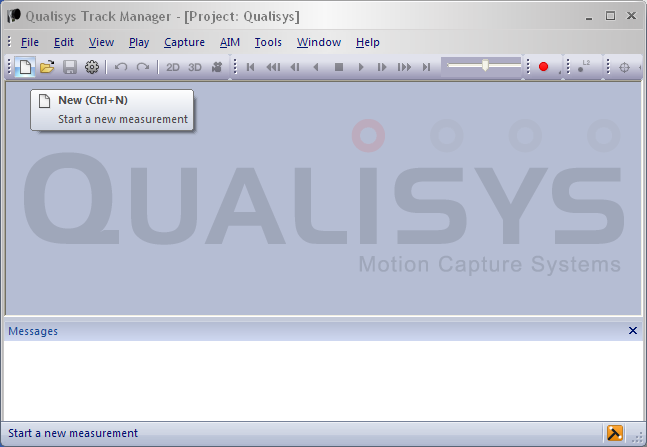
\includegraphics[width=1\textwidth]{fig/qualisys_new} 
			\caption{Qualisys Track Manager start window}
			\label{fig: Qualisys Track Manager start window}
		\end{figure}
	\item Push the white sheet icon to start a new measurement. The main window should then display the 2D view, as in Figure \ref{fig: Qualisys Track Manager 2D view}.
		\begin{figure}[!h]
			\centering 
			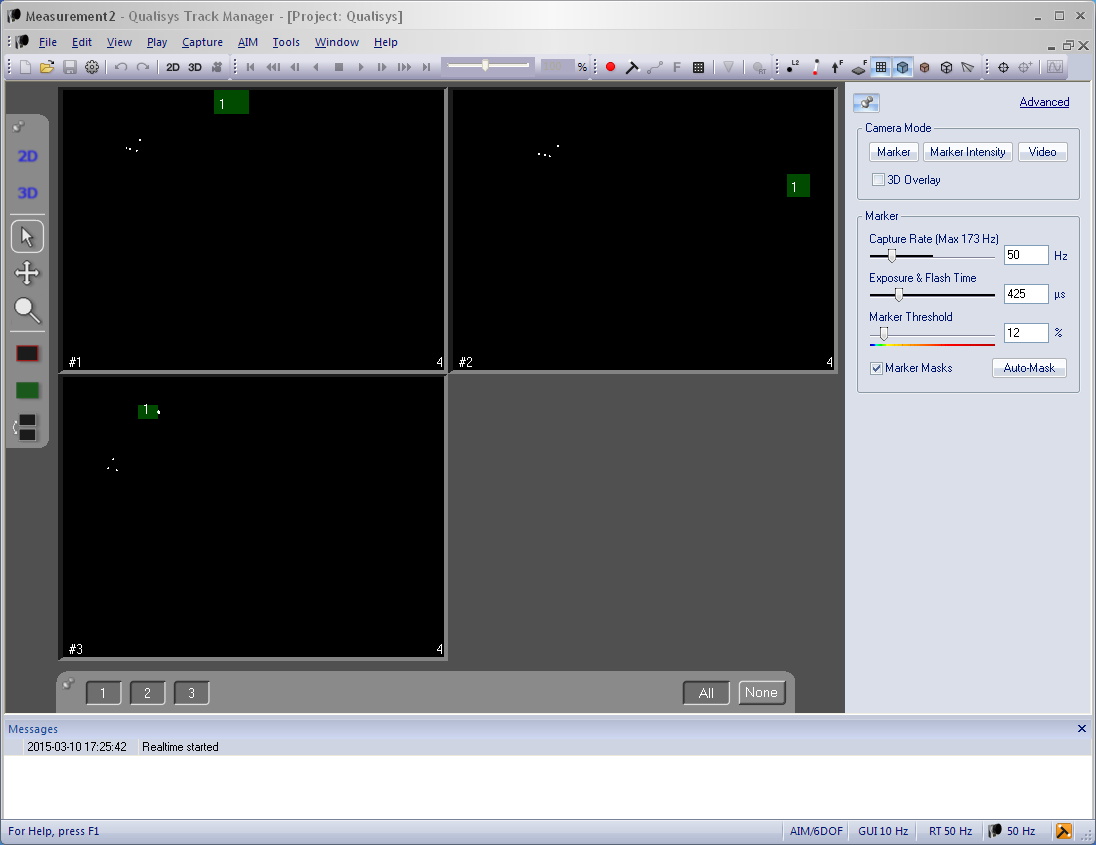
\includegraphics[width=1\textwidth]{fig/qualisys_3cams} 
			\caption{Qualisys Track Manager 2D view} 
			\label{fig: Qualisys Track Manager 2D view}
		\end{figure}
	The squares numbered \#1, \#2 and \#3 show the basin as seen from the respective cameras. The white dots are the vessel reflectors. A minimum of three reflectors must be visible in each camera. 
\end{enumerate}

\subsubsection*{Aquire body}
\begin{enumerate}
	\item Push the gear icon to access Project Options. Navigate to 6DOF Tracking,
	as in Figure \ref{fig:Qualisys-Track-Manager6DOF}.
	\begin{figure}[!h]
		\centering 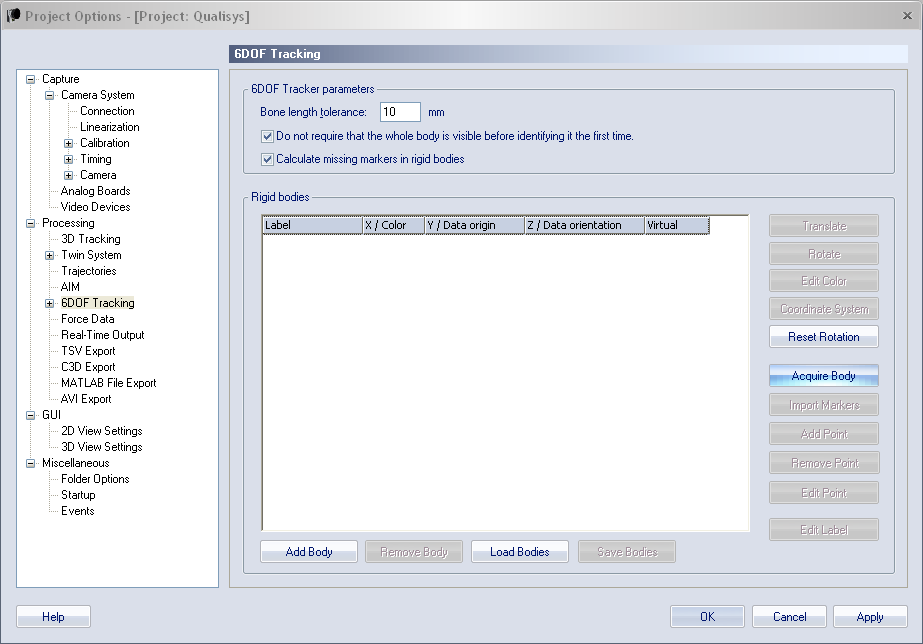
\includegraphics[width=1\textwidth]{fig/qualisys_6dof} \caption{\label{fig:Qualisys-Track-Manager6DOF}Qualisys Track Manager 6 DOF
			Tracking}
	\end{figure}
	\item Remove previous bodies, if any.
	\item Align the vessel with 0\degree heading (i.e. with the bow pointing towards the command center) and push ``Acquire Body'' to get the position of the reflectors. A list appears, as in Figure \ref{fig:Qualisys-Track-ManagerAquiredBody}. 
	\begin{figure}[!h]
		\centering 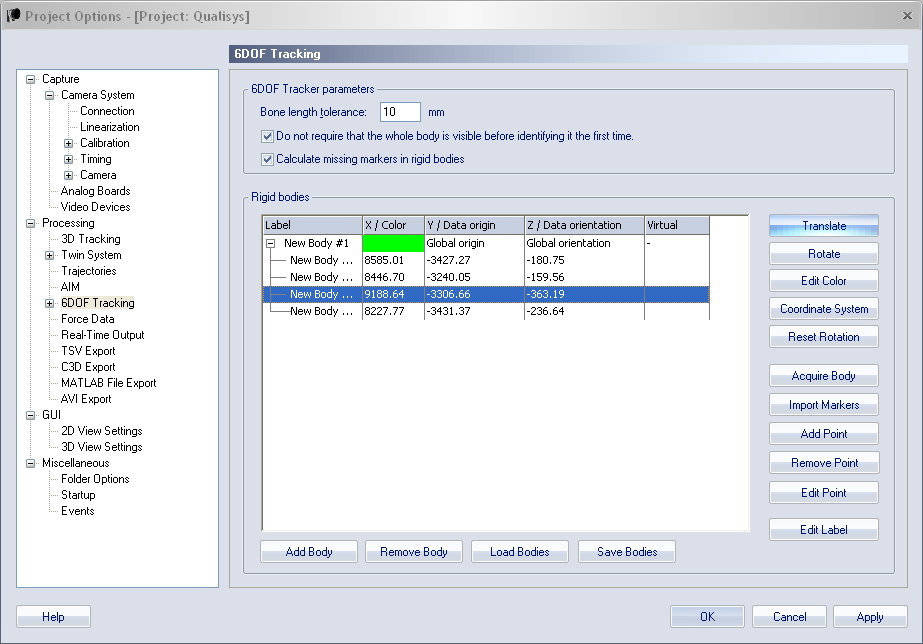
\includegraphics[width=1\textwidth]{fig/qualisys_orientating}
		\caption{Qualisys Track Manager aquired body}
		\label{fig:Qualisys-Track-ManagerAquiredBody}
	\end{figure}
	\item To redefine the body fixed coordinate frame, choose a reference reflector. As highlighted in Figure \ref{fig:Qualisys-Track-ManagerAquiredBody}, it may be practical to choose the highest-most, in this case reflector 3. Push ``Translate'' and enter the coordinates of the chosen reflector in the desired frame. See the Handbook for the specific vessel for information of the position of this reflector in the body-frame. 
	\item Verify that Qualisys is set to \textit{zyx}-convention for the rotations. In the left-pane navigation tree, expand 6DOF Tracking, select Euler Angles. Figure \ref{fig:QTM_euler} show the correct setting for \textit{zyx}-convention. 
	\begin{figure}[h!]
		\centering
		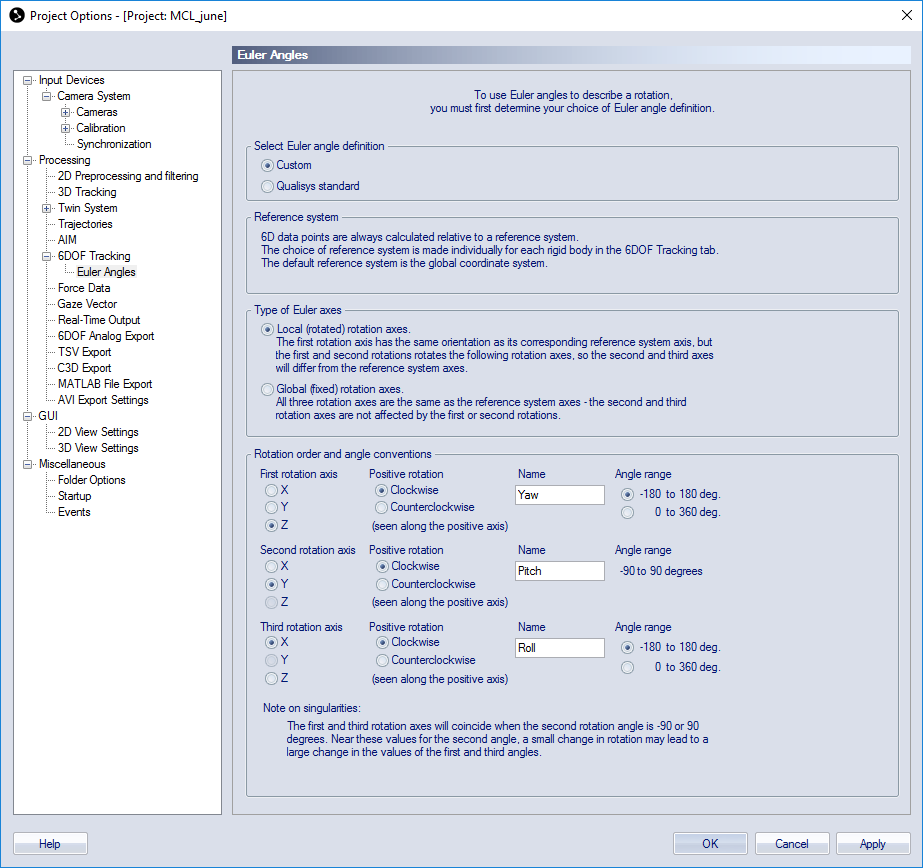
\includegraphics[width=0.8\textwidth]{fig/QTM_euler.png}
		\caption{QTM rotation convention}
		\label{fig:QTM_euler}
	\end{figure}
	\item Finally, select 3D view to confirm that the body-fixed frame is indeed located as desired, as in Figure \ref{fig:Qualisys-Track-Managerr3D}.
	\begin{figure}[!h]
		\centering 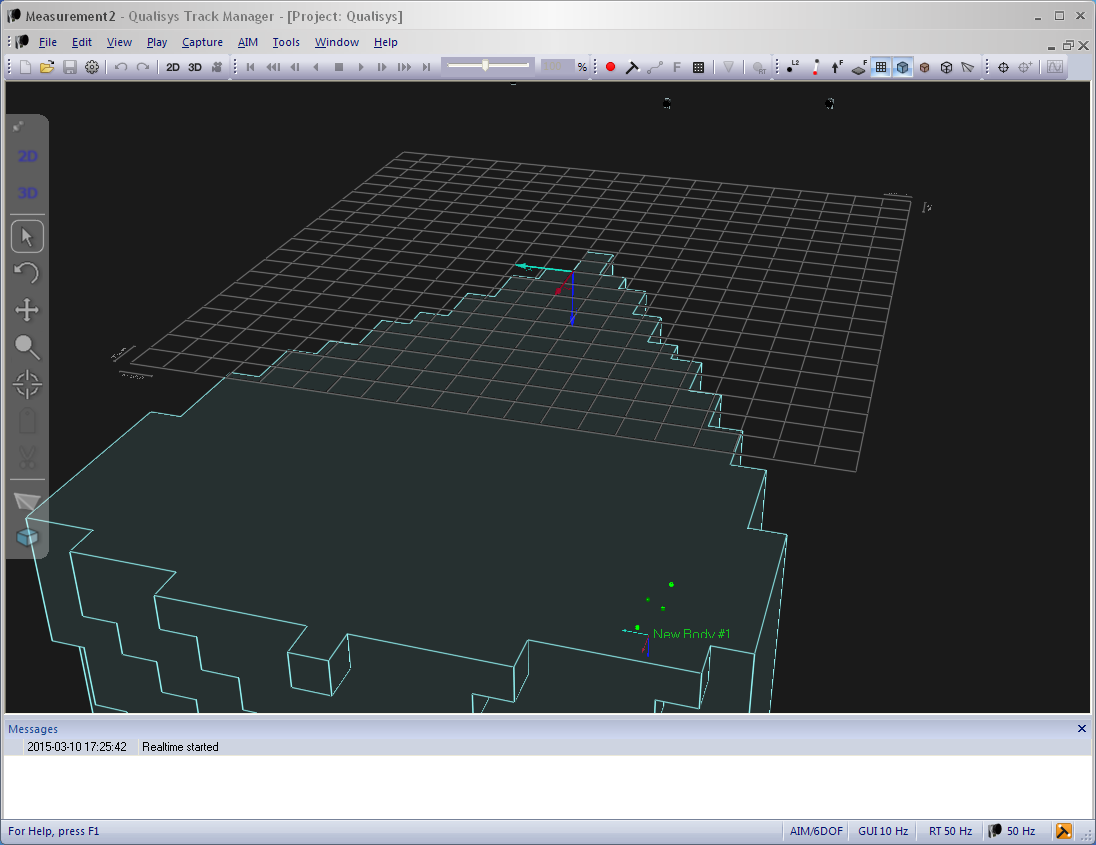
\includegraphics[width=1\textwidth]{fig/qualisys_3d} \caption{\label{fig:Qualisys-Track-Managerr3D}Qualisys Track Manager 3D view}
	\end{figure}
\end{enumerate}

\subsubsection*{Troubleshooting}
\paragraph*{Long waiting for camera}
\begin{figure}[htb!]
	\centering 
	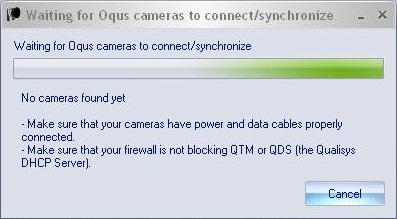
\includegraphics[scale=0.45]{fig/qualisys_waiting_to_connect}
	\caption{Qualisys Track Manager waiting for cameras}
	\label{fig:Qualisys-Track-ManagerWaiting}
\end{figure}
If the operation depicted in Figure \ref{fig:Qualisys-Track-ManagerWaiting} is unsuccessful after a couple of minutes, reboot the cameras by unplugging and reconnecting the power cord on the rack.
\paragraph*{Reflectors visible in 2D, but not in 3D window}
When aqcuiring the body, the vessel must be in the calibrated area for the cameras. If the reflectors are visible for all 3 cameras in 2D visualization, but not in 3D visualization, verify that the vessel is placed inside the calibrated area. In 3D, on the left pane, press the box and choose to show calibrated area, as illustrated in Figure \ref{fig:calibrated_area}
\begin{figure}[htb!]
	\centerline{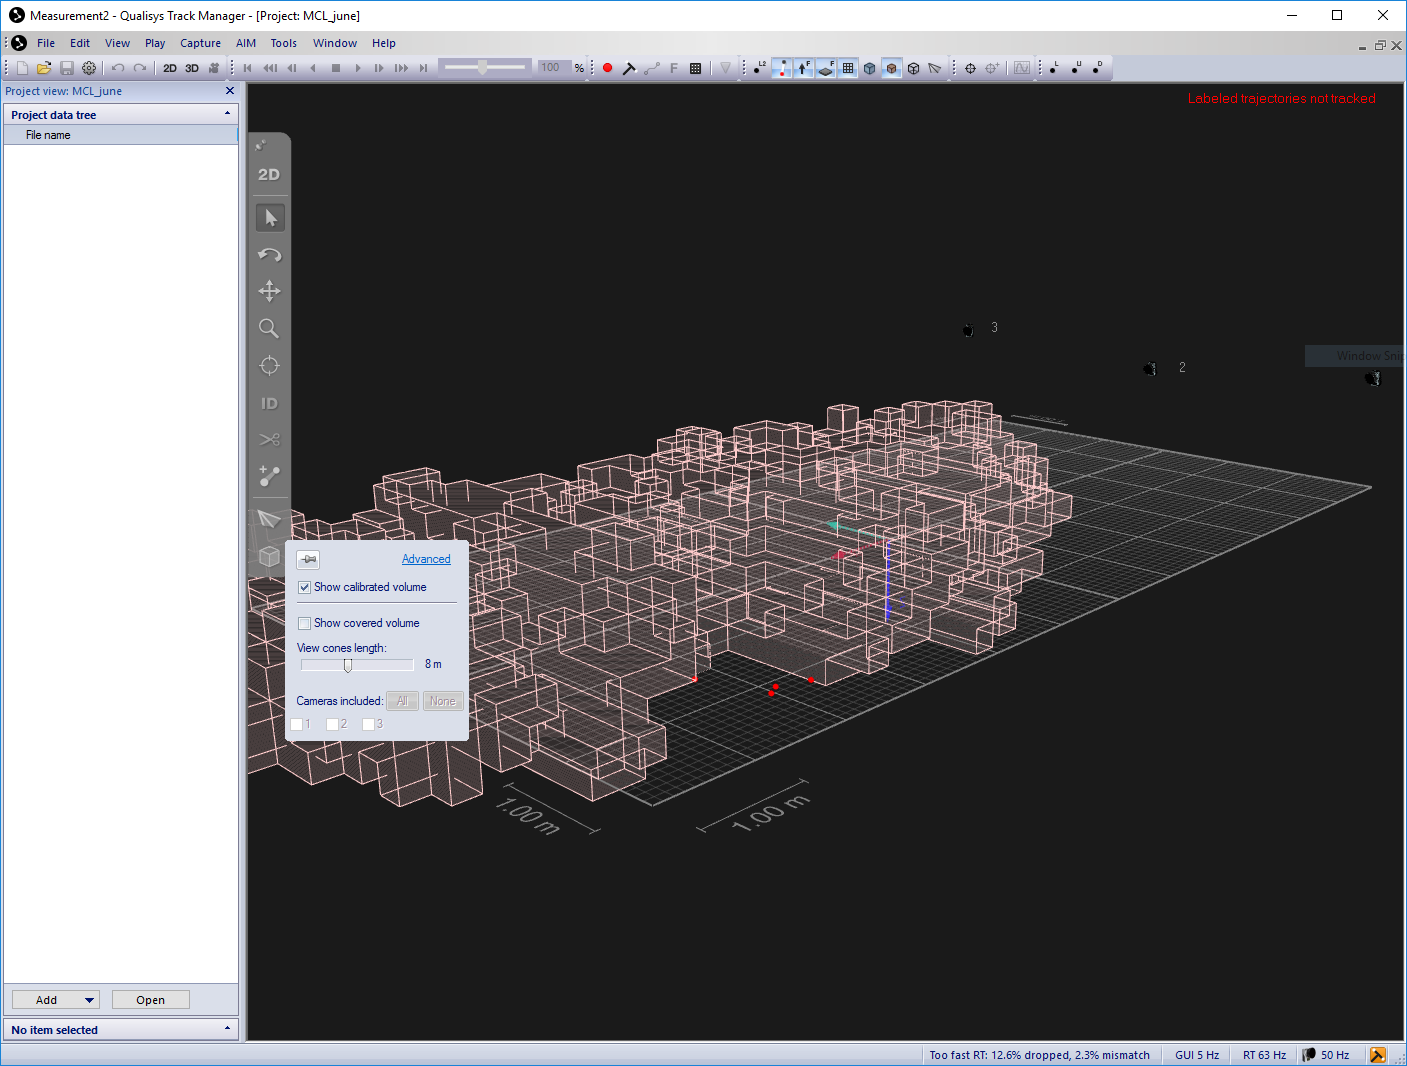
\includegraphics[scale=0.4]{fig/calibrated_area.png}}
	\caption{QTM calibrated area}
	\label{fig:calibrated_area}
\end{figure}
\clearpage{}
\subsection{Importing Data from the Qualisys System into ROS and MATLAB(Linux)}
The following approach may be used to read Qualisys data into ROS and MATLAB. The method is convenient for Qualisys data into to MATLAB independent on whether the rest of the system use ROS or not. The method, as described is limited to Linux-operating systems.

The first part of the manual describe how import Qualisys data into ROS, while the second part describe how to get the data from ROS into MATLAB/Simulink.

Please note the following: 
\begin{itemize}
	\item In the manual, the dollar sign \$ indicate a line of text that should be written in the Linux- terminal window.
	\item In the manual gedit is used as text editor. This can be replaced with the readers favourite text editor.
	\item The manual is written and tested for ROS-Indigo and MATLAB 2015b. It is based on MATLAB's manual for importing custom messages \citep{MathWorks2016}, which is and adapted and expanded to fit that of the MC lab and the Qualisys system.
	\item You need MATLAB version 2015a or newer in order to proceed with the MATLAB section of the manual.
\end{itemize}

\subsubsection{Manual}
If not already installed on the machine you should start by installing ROS. Follow the instructions on the ROS download page: \url{http://wiki.ros.org/indigo/Installation/Ubuntu}.

You should now make a ROS workspace in your home directory:

\begin{verbatim}$mkdir -p ~/catkin_ws/src 
$cd ~/catkin_ws/src
$catkin_init_workspace\end{verbatim}

You now need to make sure that one are sourcing the setup.bash file in your ROS workspace each time you open your terminal window. This can be done by changing the bash file with the following command:

\begin{verbatim}$ echo "source ~/catkin_ws/devel/setup.bash" >> ~/.bashrc\end{verbatim}

Now import the Qualisys driver from GitHub. (The driver \citep{KumarRobotics2016} is avaiable through the Apache License )

\begin{verbatim}$ cd ~/catkin_ws/src
$ git clone https://github.com/KumarRobotics/qualisys
$ cd ~/catkin_ws
$ catkin_make\end{verbatim}

Open the qualisys.launch file in a text-editor

\begin{verbatim}$ sudo gedit ~/catkin_ws/src/qualisys/launch/qualisys.launch\end{verbatim}

Edit the ip address and port number for the Qualisys system. (As of March 2016 the IP is: 192.168.0.10 and the port is 22222 )

The driver should now be set for interfacing with Qualisys in ROS. To test it, first check that you are able to ping the Qualisys system over the MC lab WiFi.

\begin{verbatim}$ ping 192.168.0.10\end{verbatim}

If you successfully pinged the qualisys system it should now be possible to listen to the data from the Qualisys system.

(Note that the Qualisys system need to recognize the IR-markers in the MC lab in order to transmit data. It may be smart to first to check that the computer running Qualisys software in the MC-Lab sees the marker)

\begin{verbatim}$ roslaunch qualisys qualisys.launch
$ rostopic list\end{verbatim}

The command ``rostopic list'' prints the ROS active ROS topics. It should now be printed a qualisys topic in terminal. The name will depend on the name set on the Qualisys computer. In this manual the topic is named /qualisys/CSE1.

You can now listen to the data as it is published to ROS

\begin{verbatim}$ rostopic echo /qualisys/CSE1\end{verbatim}

\subsubsection{Getting Qualisys data to MATLAB}

The message sent from the Qualisys system is a custom message that MATLAB does not recognize (most messages in ROS is not custom, and will be recognized by MATLAB). In order to get the Qualisys data into MATLAB you one to facilitate so that MATLAB recognize the custom message.

Start by creating a new folder \textasciitilde{}/qualisysDir. Now copy the folder named qualisys, located in \textasciitilde{}/catkin\_ws/src and paste it into the folder \textasciitilde{}/qualisysDir

Now one want to edit the package file so that MATLAB recognizes the messages.

\begin{verbatim}Sudo gedit ~/qualisysDir/qualisys/package.xml\end{verbatim}

Add the following two lines somewhere in the main body of the package.xml file.

\begin{verbatim}<build_depend>geometry_msgs</build_depend>
<build_depend>std_msgs</build_depend>\end{verbatim}

Now open MATLAB. The first step in MATLAB is to download the ROS custom message package. Type the following lines into the MATLAB command window, and follow instructions to download the ROS custom message package.

\begin{verbatim}roboticsAddons (in MATLAB 2016)
roboticsSupportPackages  (in MATLAB 2015)\end{verbatim}

When the download is finished paste the following commands in the MATLAB command window.

\begin{verbatim}folderpath= '~/qualisysDir'
rosgenmsg(folderpath)\end{verbatim}

Now follow the instructions generated by MATLAB in order generate the needed message type. In this process you may need allow writing permission to the file ``pathdef.m''

You are now ready to get the data into MATLAB.

Remember that the Qualisys node always need to be launched before reading signals in MATLAB.

\begin{verbatim}roslaunch qualisys qualisys.launch\end{verbatim}

You can now get the data into Simulink by the Subscriber block, or to MATLAB workspace by typing the following commands:

\begin{verbatim}Subb = rossubscriber('/qualisys/CSE1');
posedata = receive(Subb,10);\end{verbatim}

\clearpage

\section{Towing carriage}
\begin{figure}[htb!]
	\centering 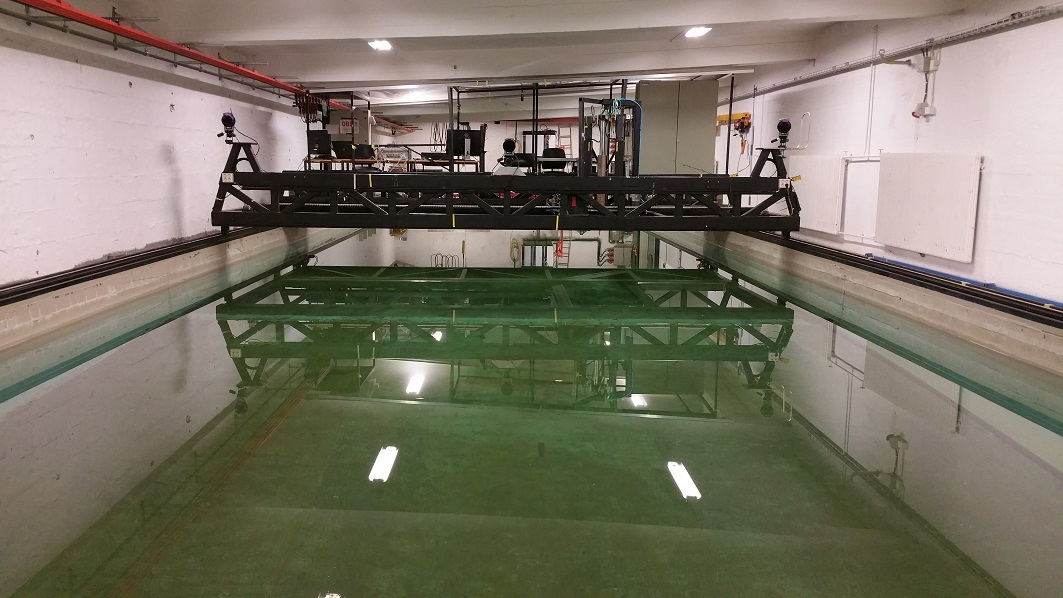
\includegraphics[width=1\textwidth]{fig/towing_carriage}
	\caption{Towing carriage}
	\label{fig: Towing carriage}
\end{figure}
The scope of this section is to explain how to safely operate the carriage without any damage towards humans or equipment. 

\subsection{Preparation before startup}
To start with, you must make sure that any items mounted or fixed to the carriage are securely fitted, so they don't prevent the operation of the carriage. All personnel must stay on the operation platform during the travel of any axis.

Locate the Emergency Button and place it so that you can easily reach it from where you are sited. DO NOT USE THE EMERGENCY BUTTOM AS A BRAKE. YOU MUST ONLY OPERATE IT WHEN YOU ARE IN REAL EMERGENCY SITUATIONS.

\subsubsection*{Operation console}
\begin{figure}[htb!]
	\centering 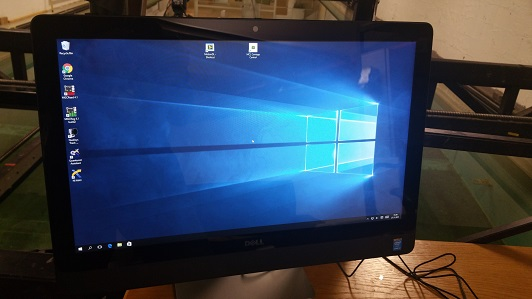
\includegraphics[width=0.8\textwidth]{fig/towing_console}
	\caption{Towing console}
	\label{fig: Towing console}
\end{figure}

The operation console is an All-in-one PC. The Power button is on the bottom right side of the screen. If the operation panel is not on the desktop, you can start it by double clicking on desktop Icon, shown in Figure \ref{fig: Towing console}.

\subsection{Manual Operation of the Carriage}
\subsubsection*{Setup}
\begin{figure}[htb!]
	\centering 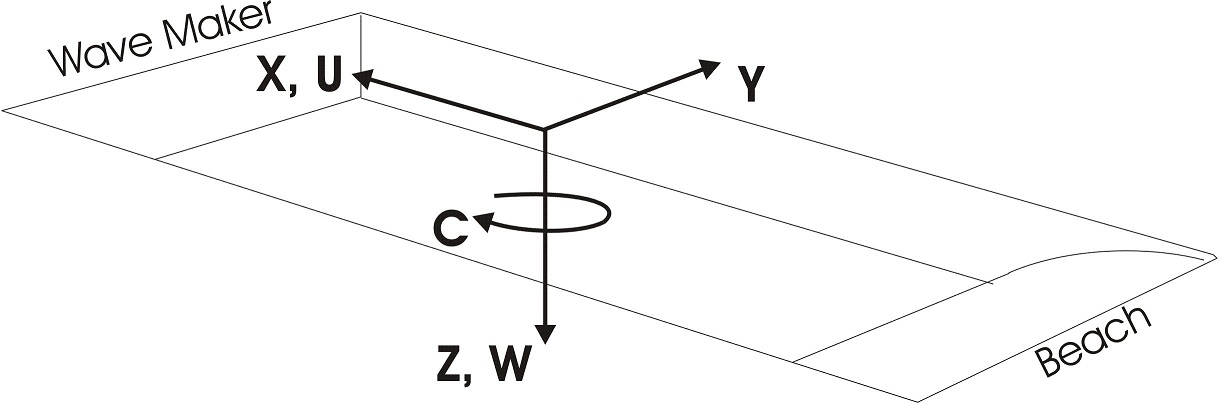
\includegraphics[width=0.8\textwidth]{fig/towing_coordinate_sketch}
	\caption{Coordinate system}
	\label{fig: Towing carriage-1}
\end{figure}

\begin{figure}[htb!]
	\centering 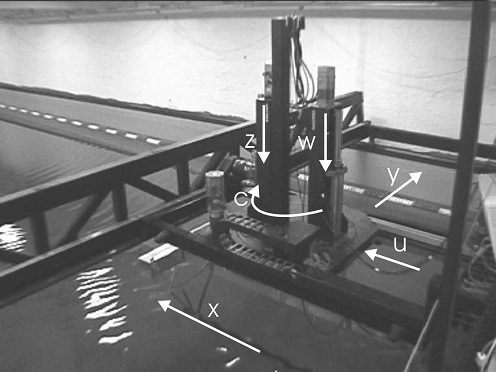
\includegraphics[width=0.8\textwidth]{fig/towing_coordinate_photo}
	\caption{Coordinate system}
\end{figure}

\begin{table}
	\centering{}%
	\begin{tabular}{lllllll}
		\hline 
		& \multicolumn{2}{l}{Forward/Backward} & \multicolumn{2}{l}{Acceleration} & \multicolumn{2}{l}{Position}\tabularnewline
		Axis & \multicolumn{2}{l}{Speed} & \multicolumn{2}{l}{Deceleration} & \multicolumn{2}{l}{Pos./Neg. Limit}\tabularnewline
		\hline 
		X & 0 - 2.0 & {[}m/s{]}  & \% of 0 - 0.5 & $\text{m/\ensuremath{s^{2}}}$ & 0 - 22 & {[}m{]}\tabularnewline
		Y & 0 - 1.0 & {[}m/s{]}  & \% of 0 - 1.0 & $\text{m/\ensuremath{s^{2}}}$ & 0 - 4.5 & {[}m{]}\tabularnewline
		U & 0 - 1.0 & {[}m/s{]}  & \% of 0 - 1.0 & $\text{m/\ensuremath{s^{2}}}$ & 0 - 1 & {[}m{]}\tabularnewline
		C & 0 - 10  & {[}deg/s{]} & \% of 0 - 20 & $\text{deg/\ensuremath{s^{2}}}$ & 0 - 255 & {[}deg{]}\tabularnewline
		Z & 0 - 1.0 & {[}m/s{]}  & \% of 0 - 2.0 & $\text{m/\ensuremath{s^{2}}}$ & 0 - 0.5 & {[}m{]}\tabularnewline
		W & 0 - 1.0 & {[}m/s{]}  & \% of 0 - 2.0 & $\text{m/\ensuremath{s^{2}}}$ & 0 - 0.5 & {[}m{]}\tabularnewline
		\hline 
	\end{tabular}\caption{\label{tab: Operation Limit}Operation Limit}
\end{table}

\begin{figure}[htb!]
	\centering 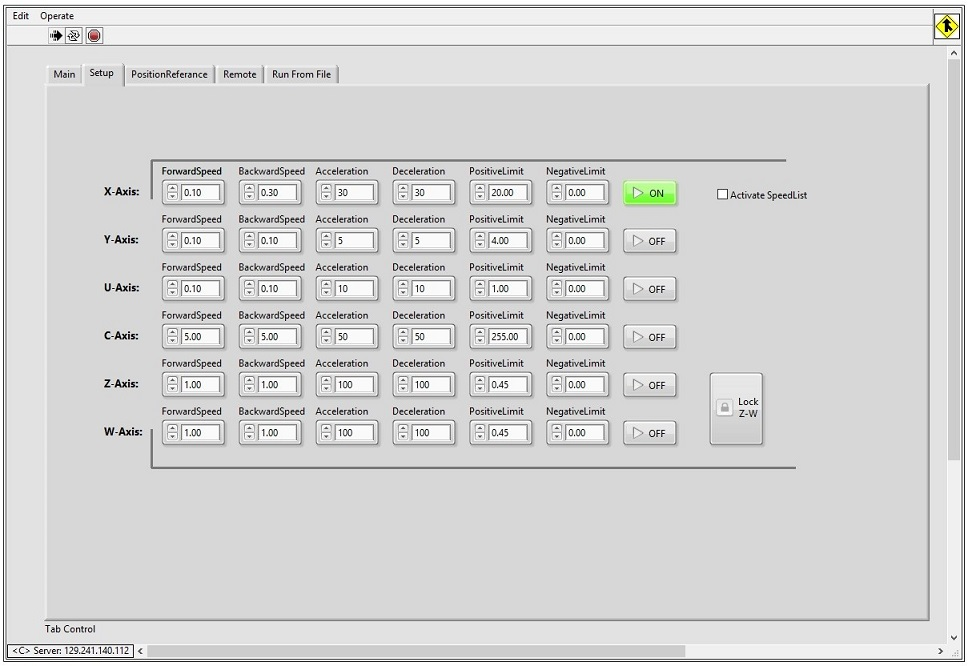
\includegraphics[width=0.8\textwidth]{fig/towing_parameteres}
	\caption{Setup}
	\label{fig: Towing parameters}
\end{figure}

It is very important to select the Setup tab first before you start any operation of the carriage. As you can see in Figure \ref{fig: Towing parameters}, it is possible to change the travel parameters for all available axes. In principle, all axis parameters have different range limits. These are listed in Table \ref{tab: Operation Limit}.

All axes can be activated or deactivate by using the ON button.

For the X axis it is possible to activate a list of predefined Forward speeds. You will then have the ability to automatically change to a different speed on the next run. The list can be edited in the Main Tab Window.

By selecting the ``Lock Z-W'' button the Z-W axis will operate in parallel. They will use the Z-axis parameter setup.

\subsubsection*{Main/Standard Operation}
\begin{figure}[htb!]
	\centering 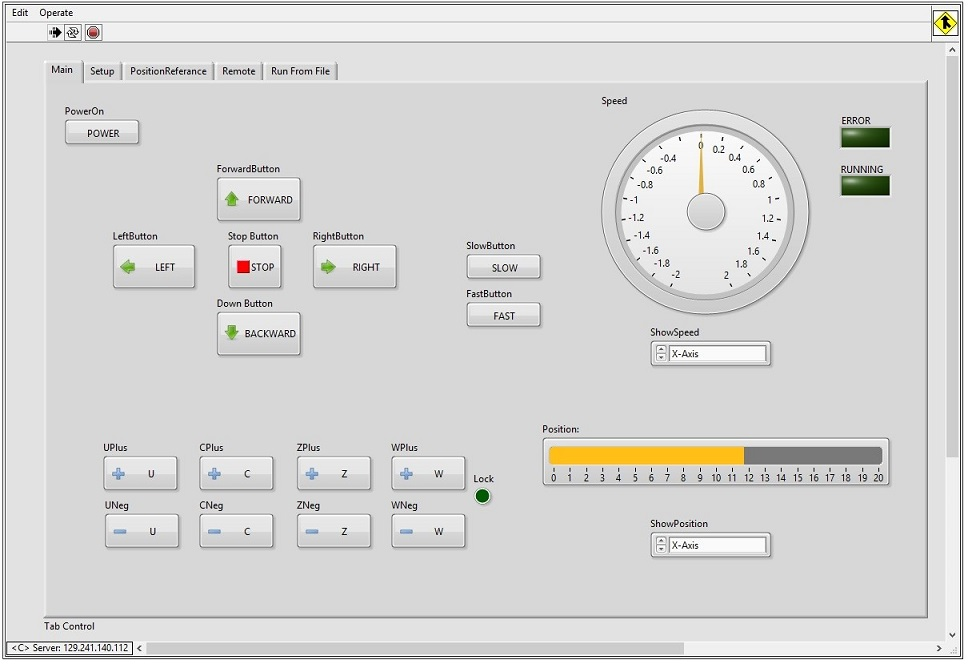
\includegraphics[width=0.8\textwidth]{fig/towing_main} 
	\caption{Main}
	\label{fig: Towing main}
\end{figure}

All the activated axes will operate within the limits set in the Setup. Only one axis can operate at a time. If you hit the button for another axis than the running one, it will instantly stop and new one will start running. To stop the running axis, simply hit the stop button. If no buttons are operated carriage axis will run it hit limit position of the current axis.

If an error occurs, for some reason, it can be cleared by hitting the ``Power'' button. If the error keeps reoccurring, please look at the Troubleshooting section of this document or contact responsible MC Lab personnel.

The current speed and position of the active axis are displayed referred to the selected limits.

\subsection{Operation Controlled automatically from PC}

\begin{figure}[htb!]
	\centering 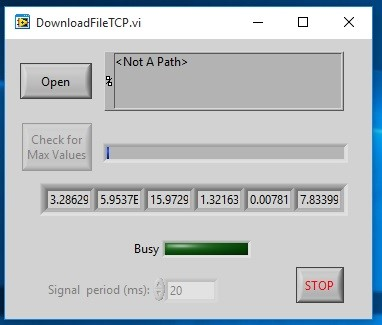
\includegraphics[width=0.8\textwidth]{fig/towing_runfromfile}
	\caption{Run From File}
	\label{fig: Towing main-1}
\end{figure}


\subsubsection*{The Trajectory Input File}

All trajectories must be defined in a .mcl input file. The format of the file is slightly more general than allowed here and is the same as for the sloshing rig input. The entries in the file are
\begin{enumerate}
	\item Time Step in ms, double precision integer (int32). Must be set to 10.
	\item Number of channels, double precision integer (int32). Must be 6.
	\item Position references in sequence: X(1),Y(1),U(1),C(1),Z(1),W(1), X(2),Y(2), double precision real (float32).
\end{enumerate}
The following MTALAB lines write the matrix body (6xN) to file on
the correct format:
\begin{verbatim}
fid=fopen(filename,'wb');
head=[10;6];
count=fwrite(fid,head,'int32');
count=count+fwrite(fid,body,'float32');
fclose(fid); 
\end{verbatim}

The resulting input file must be transferred to the realtime computer at /home/ntuser/inputpos.mcl. Normally this is done automatically when the Load button on the LabVIEW GUI is pressed. 

\begin{figure}[htb!]
	\centering 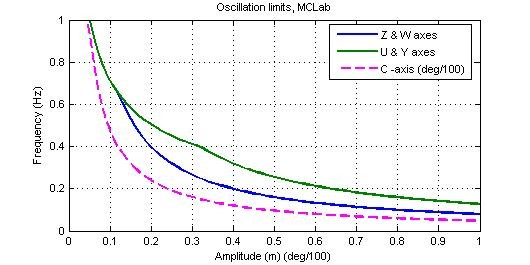
\includegraphics[width=0.8\textwidth]{fig/towing_ampvsfreq}
	\caption{\label{fig: Towing main-1-1}Operation Limit Amplitude vs. Frequency}
\end{figure}
\subsection{Troubleshooting}
\subsection{Note}
When the wagon is moving, no one is allowed to move on the sides of the basin.
\clearpage{}

\section{Wave Generator}\label{sec:wave_generator}
The wave maker is a single paddle wave making machine with a width of 6 meter and it is equipped with an Active Wave Absorption Control System (AWACS 2). The single paddle wave generator is controlled by a dedicated computer. The machine can produce both regular and irregular waves because of the DHI Wave Synthesizer the system has. Available spectrum are first order Stoke, JONSWAP, Pierson-Moskowitz, Bretschneider, ISSC and ITTC. Table \ref{tab:Wave generator capacity-1} summarizes the generation capacity.
\begin{table}[h!]
	\centering{}
	\begin{tabular}{lll}
		\hline 
		& Height {[}m{]} & Period T {[}s{]}\tabularnewline
		\hline 
		Regular waves & $H<0.25$ & 0.3 - 3.0\tabularnewline
		Irregular waves & \textbf{$H_{s}<0.15$} & 0.6 - 1.5\tabularnewline
		\hline 
	\end{tabular}\caption{\label{tab:Wave generator capacity-1}Wave generator capacity}
\end{table}
\subsection{User Manual}
\todo{Add a description on how to use the system once the NEW wave generator is installed(fall 2017)}
\clearpage{}
\section{Video-Camera System}
The laboratory is equipped with 2 high-resolution cameras for recording of activity in the basin, one on each side. The cameras are remotely operated from a dedicated PC in the command center using the \textit{Intelligent Video Management System 4200 (iVMS-4200 client)} software. The computer is located on the floor, is connected to the TV-monitor mounted on the wall, and has wireless mouse and keyboard(labeled \textit{Camera system}). The software user-interface is illustrated in Figure \ref{fig:userinterface_iVMS-4200}. 

The manual control of the cameras are found in the \textit{PTZ Control} tab. The cameras feature auto-tracking of objects, which is enabled by right-clicking in the video window. The menu is illustrated in Figure \ref{fig:userinterface_iVMS-4200}, with highlighted options for auto-tracking and manual control of the camera position. 
The camera system also support recording. Note that the recorded files are large, typically several GB for some minutes of recorded video. Hence, the files should be \textit{moved} to a USB-disk(and not copied). The recorded files are found in the path: \path{C:\ivms4200\video\RecordFile\YYYYMMDD}.
\begin{figure}[htb!]
	\centerline{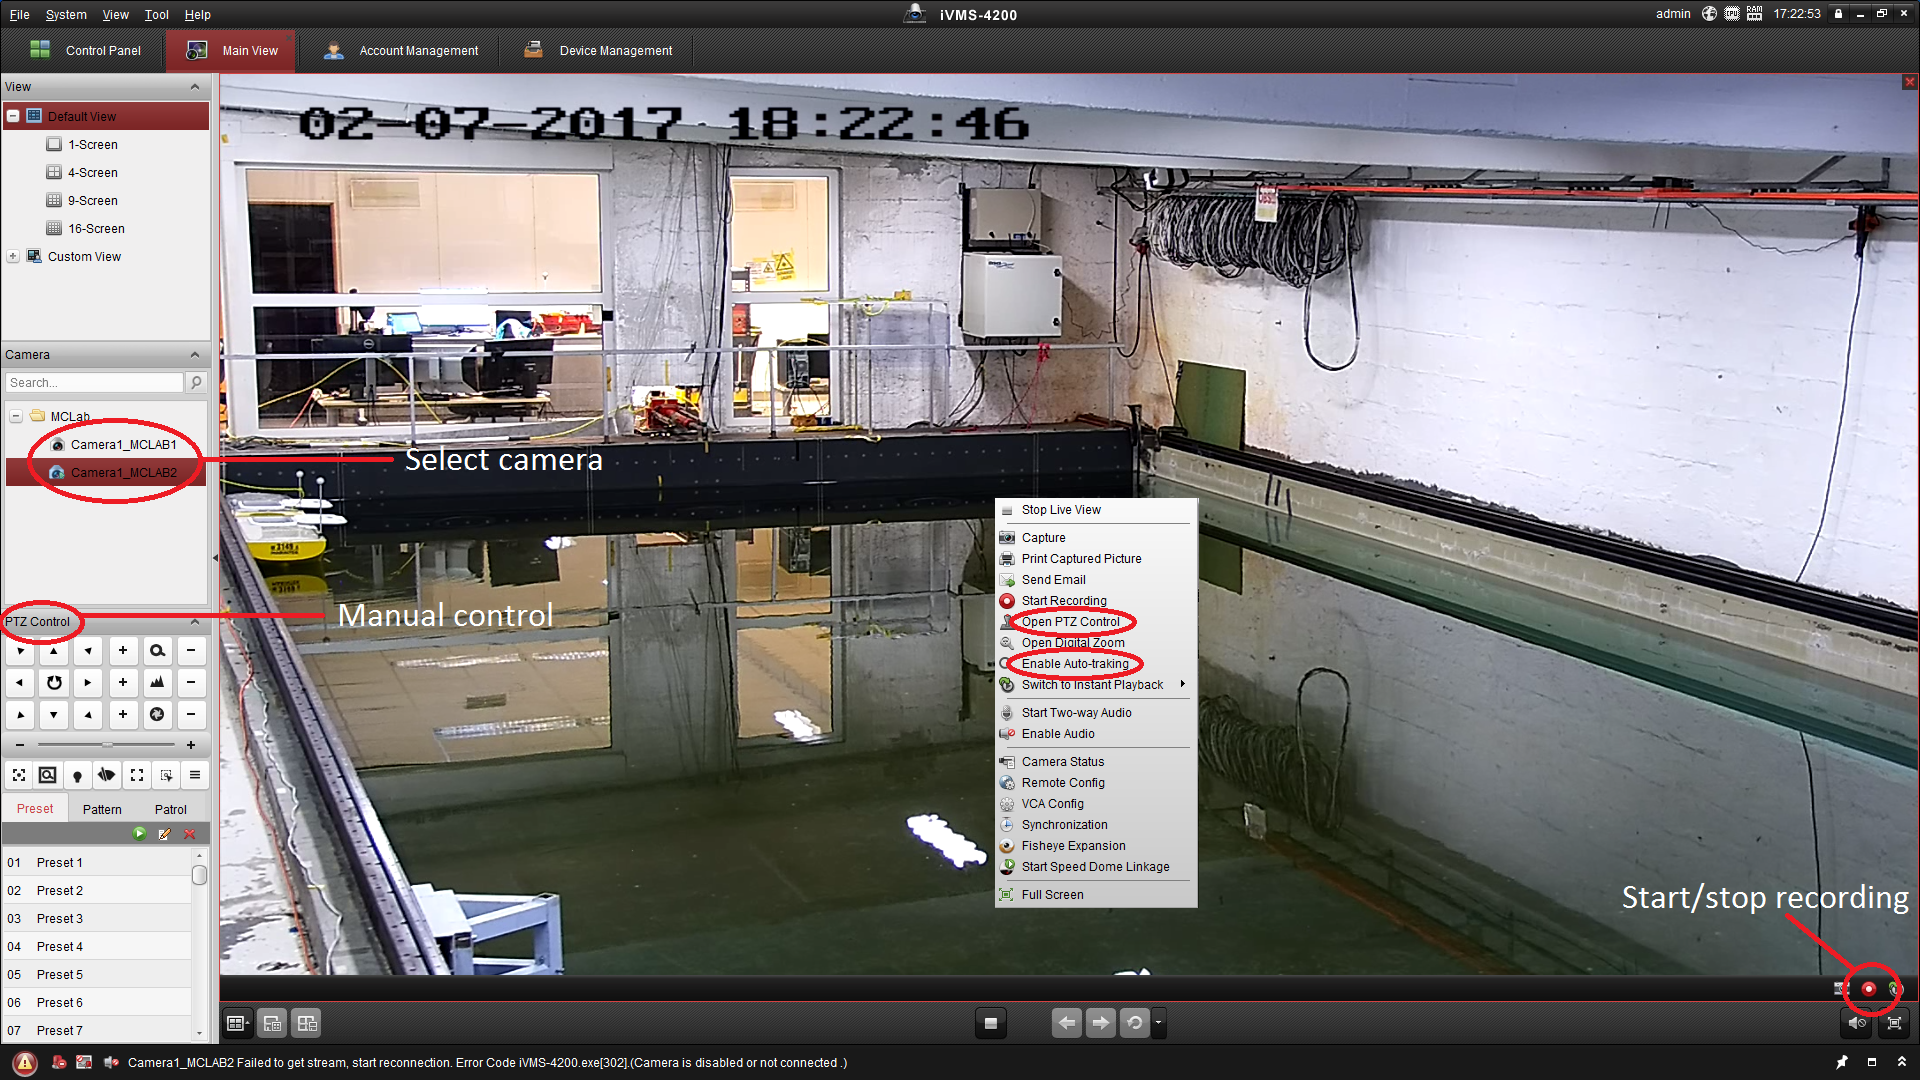
\includegraphics[width=1.4\linewidth]{fig/Camera_userinterface.png}}
	\caption{User interface iVMS-4200 camera system}
	\label{fig:userinterface_iVMS-4200}
\end{figure}

\chapter{Software}\label{ch:software}
\section{Laptop}
As of July 2017, there is a Virtual Machine with all necessary software installed. To use cRIO, the following software is needed: 
\begin{itemize}
	\item LabVIEW Full Development system, with the following modules: 
	\begin{itemize}
		\item LabVIEW Real-Time Module
		\item LabVIEW FPGA Module
		\item NI-RIO driver
	\end{itemize}
	\item MATLAB and Simulink
	\item VeriStand with all modules included in the installation file(especially NI VeriStand Model Framework)
	\item WindRiver GNU Toolchain that supports VxWorks. 
\end{itemize}
Version compatibility is an important issue, see \url{http://digital.ni.com/public.nsf/allkb/10BBA745CD5A2FAE86257F9A0054FF71}. The Virtual Machine has LabVIEW 2017, VeriStand 2017 and Matlab 2016b installed. For use of CS Enterpris 1 or CS Arctic Drill Ship, it is highly recommended to use the Virtual Machine in stead of installing all the software. To use the Virtual Machine, install VirtualBox and copy the Virtual Machine from one of the LAB-computers, or contact Hans-Martin Heyn for a copy. 

However, if installing the software, it is recommended to install the different software parts in the order given above. The installation files are found on the webpage of National Instruments, and the product key is found on \url{software.ntnu.no}. 
\section{cRIO}
Updating and changing software on cRIO is done in NI MAX. In order to update the cRIO(e.g. updating to a newer version), follow this procedure: 
\begin{enumerate}
	\item Make sure the cRIO and the laptop are on the same network(either both connected to MCLab or by an Ethernet cable)
	\item Open NI MAX. In the left pane, navigate to the cRIO. Press restart, and verify that the correct cRIO is restarting. 
	\item Right-click on the cRIO $\rightarrow$ Format Disk.
	\item Select "Attempt to restart into safe mode" and "Preserve the setting for all network adapters", as illustrated in Figure \ref{fig:format_crio}.
	\item When successfully formated, install software. Expand the cRIO, right-click on Software and select Add/Remove Software. See Figure \ref{fig:crio_install_software}
	\item Select NI CompactRIO *Version* $\rightarrow$ Next $\rightarrow$ Next $\rightarrow$ Next. There is no need to alter the software here, NI MAX installs the recommended software for the cRIO. Press Finish
	\item Right-click on Software once more, and select Add/Remove Software. Now, select Custom software installation. Choose Yes in the warning. Navigate to NI VeriStand Engine YYYY, and choose Install the feature. Press Next $\rightarrow$ Next $\rightarrow$ Finish. See Figure \ref{fig:crio_custom_install}
	\item The cRIO has now been updated with the necessary software with the version selected. 
\end{enumerate}
\begin{figure}[htb!]
	\centering
	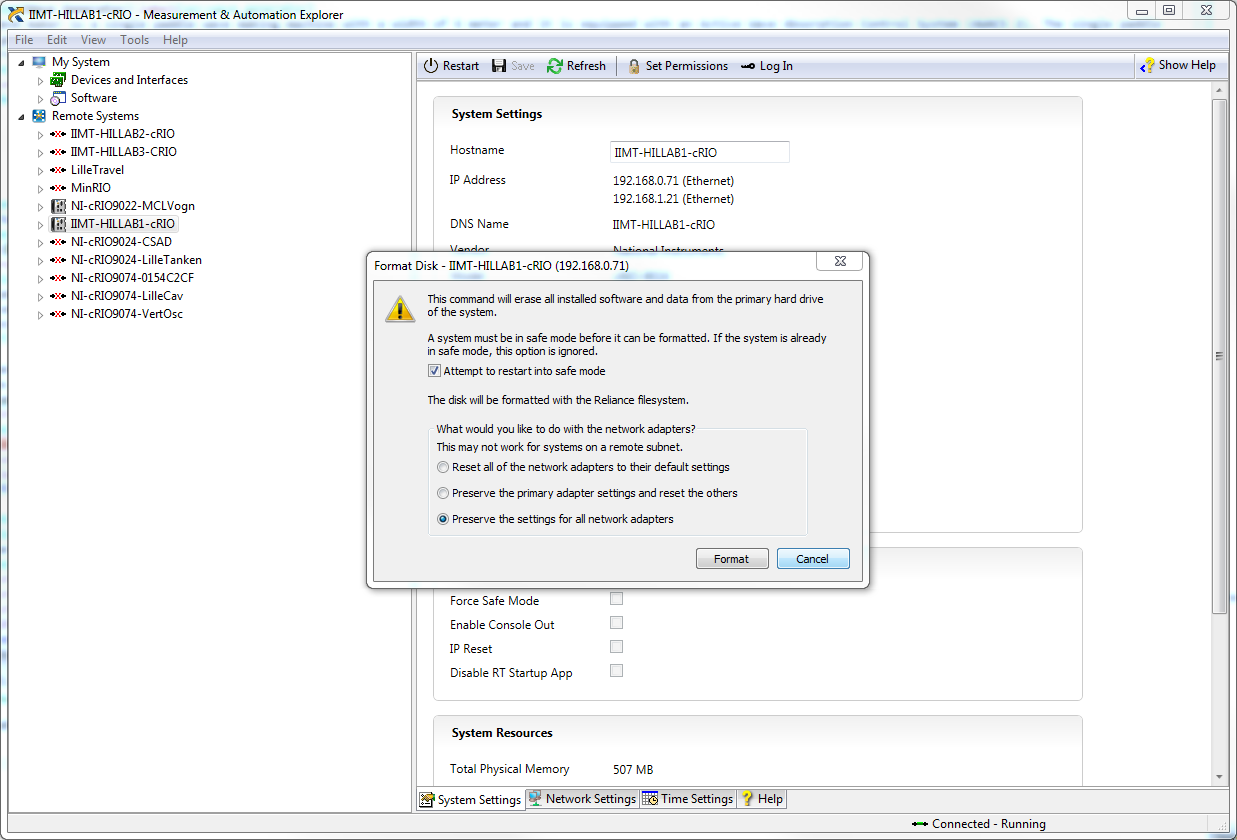
\includegraphics[scale=0.4]{fig/format_crio.png}
	\caption{Format cRIO}
	\label{fig:format_crio}
\end{figure}
\begin{figure}[htb!]
	\centering
	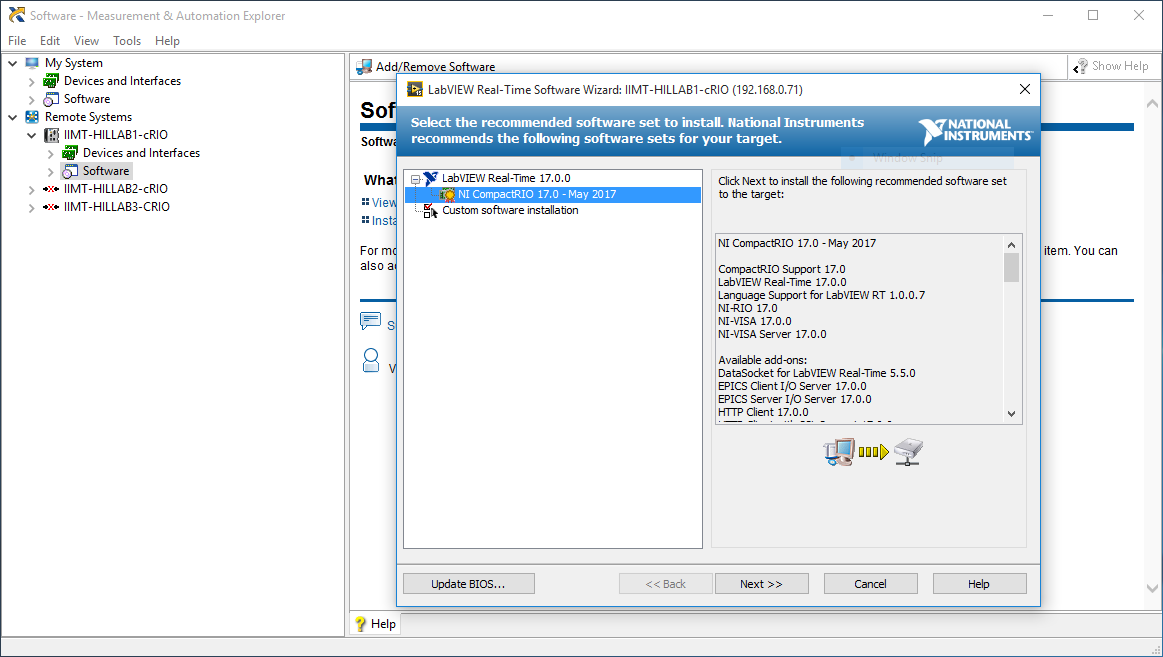
\includegraphics[scale=0.4]{fig/crio_install_software.png}
	\caption{Install software on cRIO}
	\label{fig:crio_install_software}
\end{figure}
\begin{figure}[htb!]
	\centering
	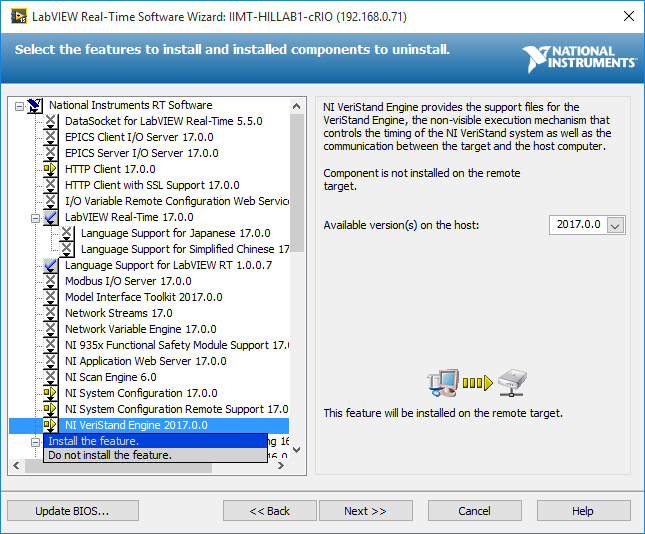
\includegraphics[scale=0.6]{fig/crio_custom_install.png}
	\caption{Install NI VeriStand Engine on cRIO}
	\label{fig:crio_custom_install}
\end{figure}

\section{Update customized simulink code}\label{sec:simulink_import}
This section describes the process of updating the customized Simulink model, and building it as a cRIO-compatible code. For illustration, the CSE1 is used here, but the process is similar for all cRIOs. First, go to GitHub and download/clone the repository related to the vehicle of interest. Then, open \textit{ctrl\_custom.slx}. The model should be similar to the one shown in Figure \ref{fig:ctrl_custom}. 
\begin{figure}[htb!]
	\centering
	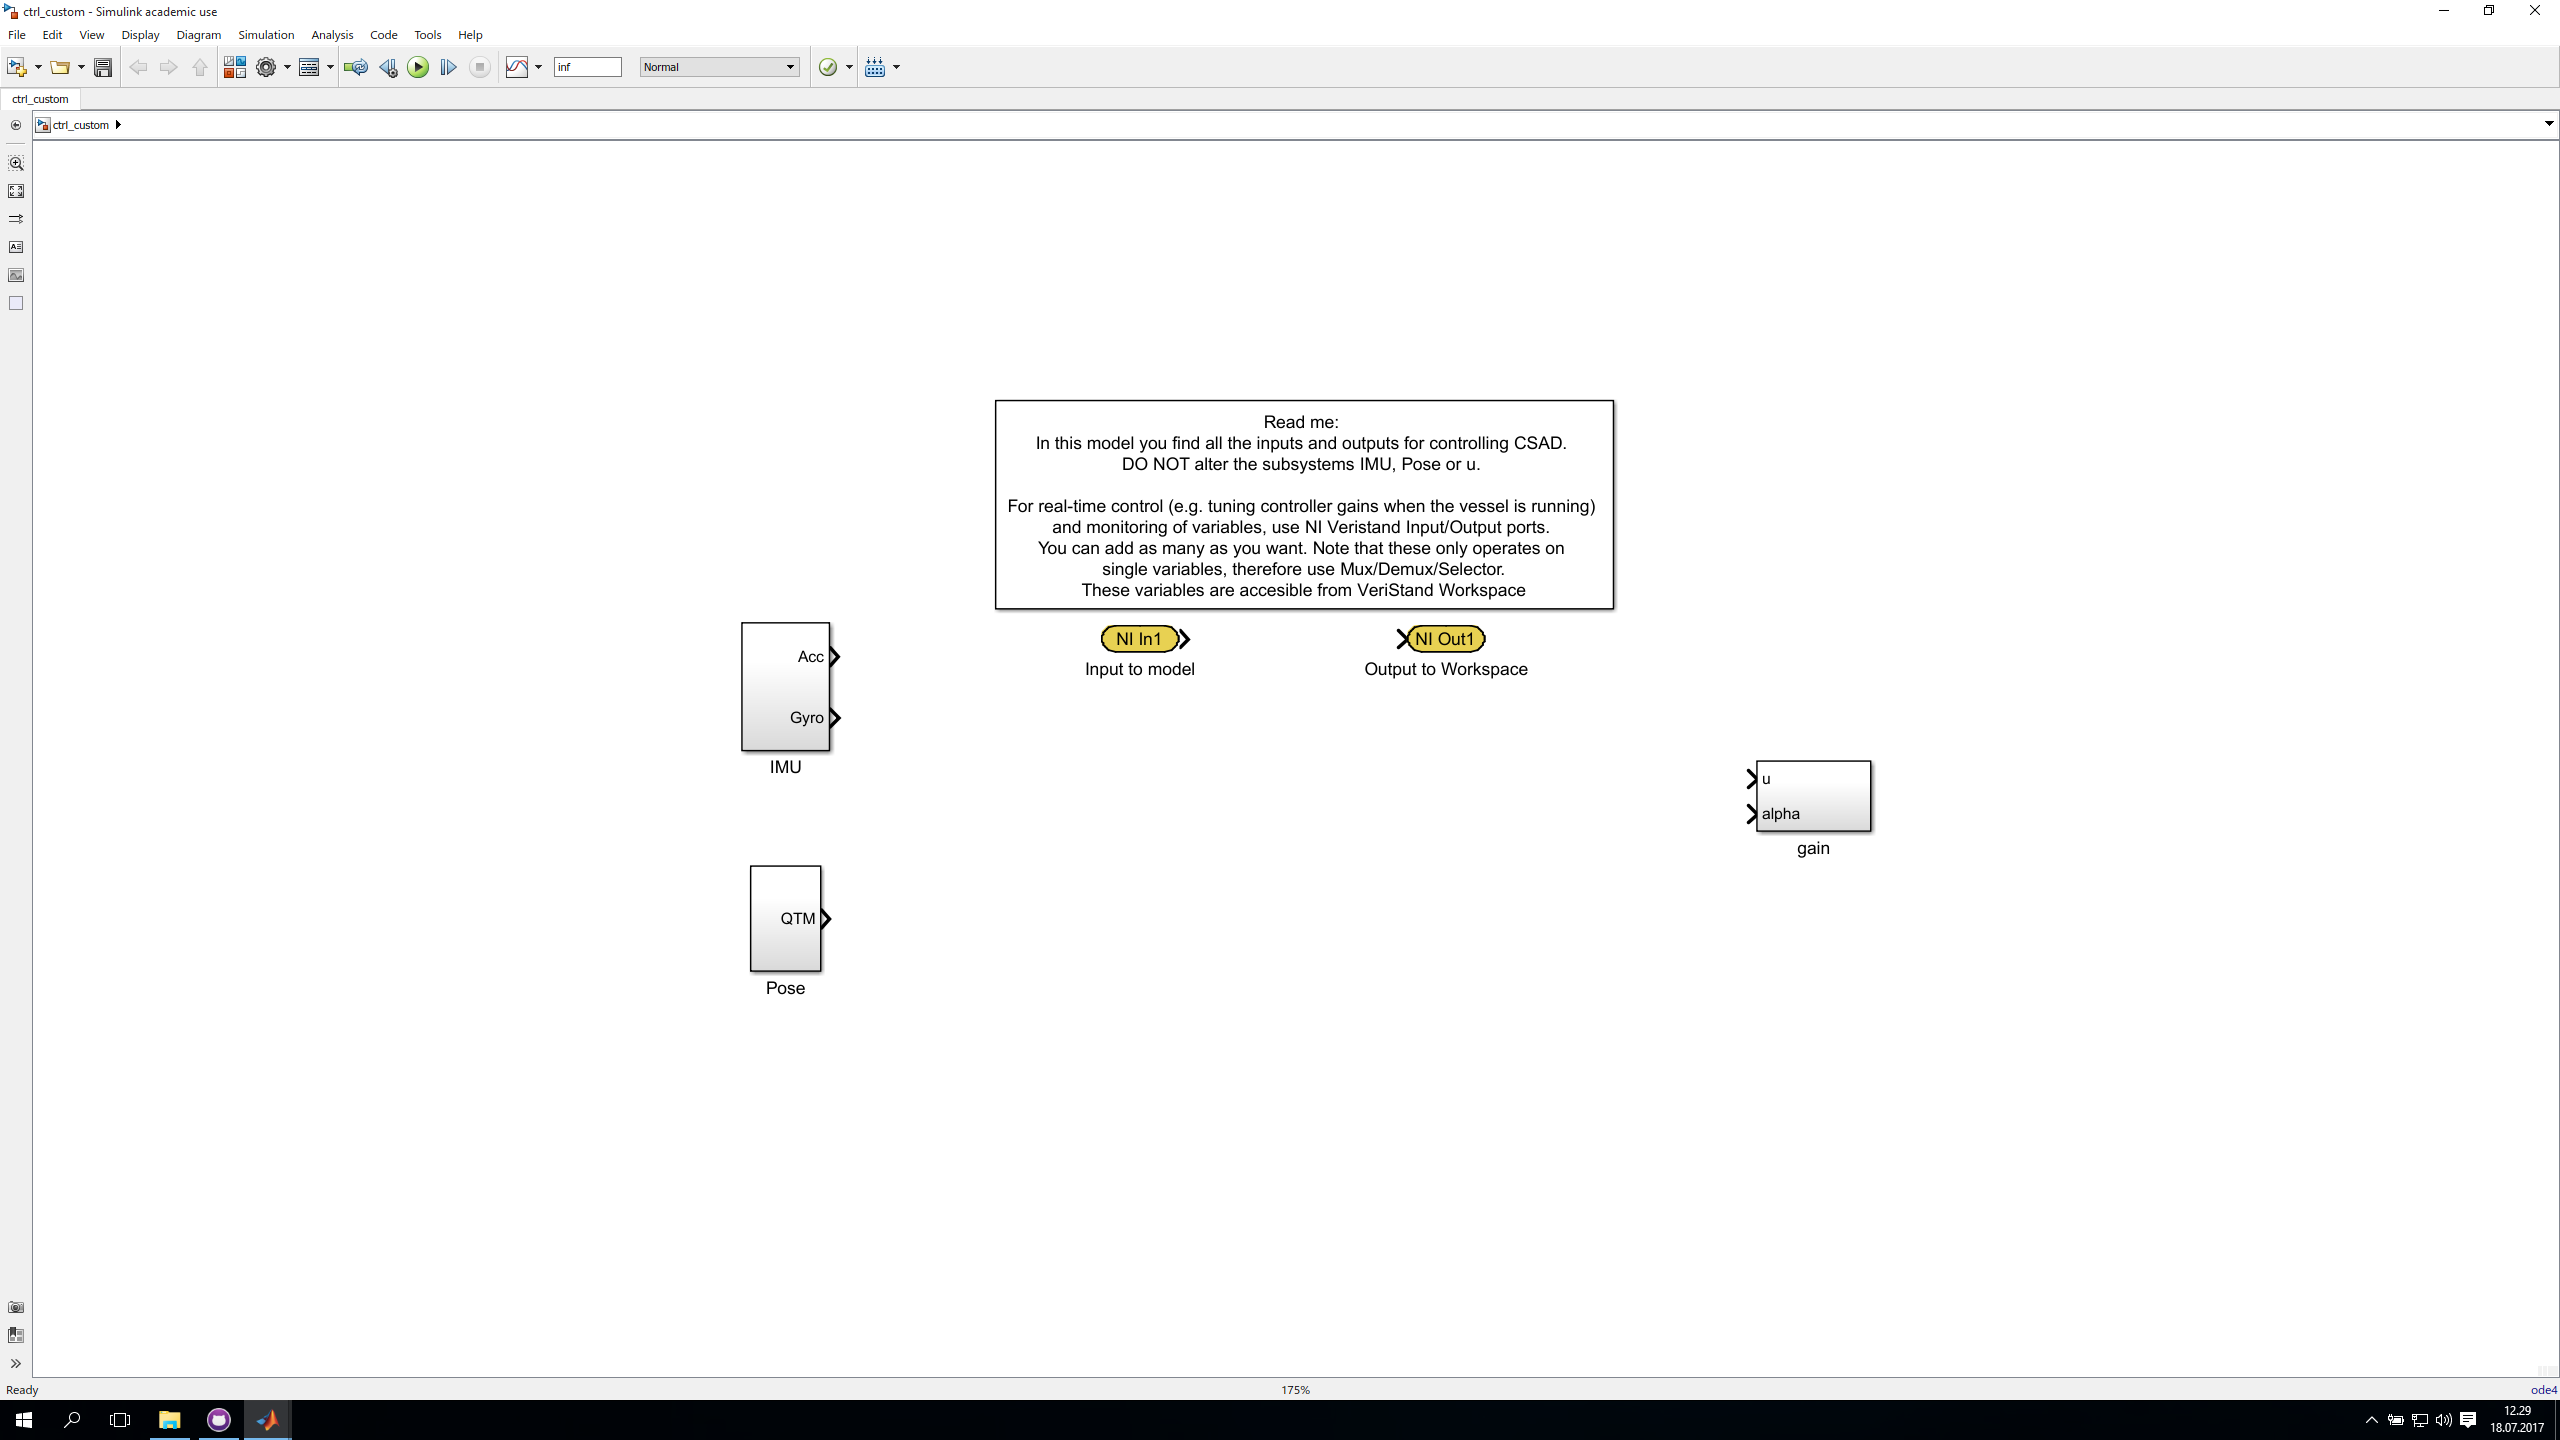
\includegraphics[width=\textwidth]{fig/ctrl_custom.png}
	\caption{ctrl\_custom.slx initial window}
	\label{fig:ctrl_custom}
\end{figure}
You should not alter the input/output subsystems, as these are already mapped properly in VeriStand. Implement your control system as desired, and include as many NI VeriStand Input/Output blocks as desired. These blocks are used to read/change parameters when the code is running on the cRIO. When the \textit{ctrl\_custom.slx} Simulink project is updated with the desired control system, the code must be compiled to C-language for exporting to the cRIO. First, make sure the active folder directory in MATLAB is \path{CSE1\simulink system\}. In Simulink, open the Model Configuration (press 
\includegraphics[scale=0.7]{fig/model_conf.png}), and make sure the following settings are applied(see Figure \ref{fig:model_configuration}):
	\begin{description}
		\item [{Solver:}] Stop time: \textbf{inf}, Solver type: \textbf{Fixed-step}, Solver: \textbf{discrete} or \textbf{ode3}, Fixed-step size: \textbf{0.01}
		\item [{Code Generation:}] System target file: \textbf{NIVeriStand\_VxWorks.tlc}. If another file is shown, press Browse and find the correct one. 
		\item [{Code Generation/NI Configuration:}] WindRiver GNU Path: \path{C:\gccdist\supp\setup-gcc.bat}. If \path{supp} does not work, change it to \path{supplemental}.
	\end{description}
	\begin{figure}[htb!]
		\centerline{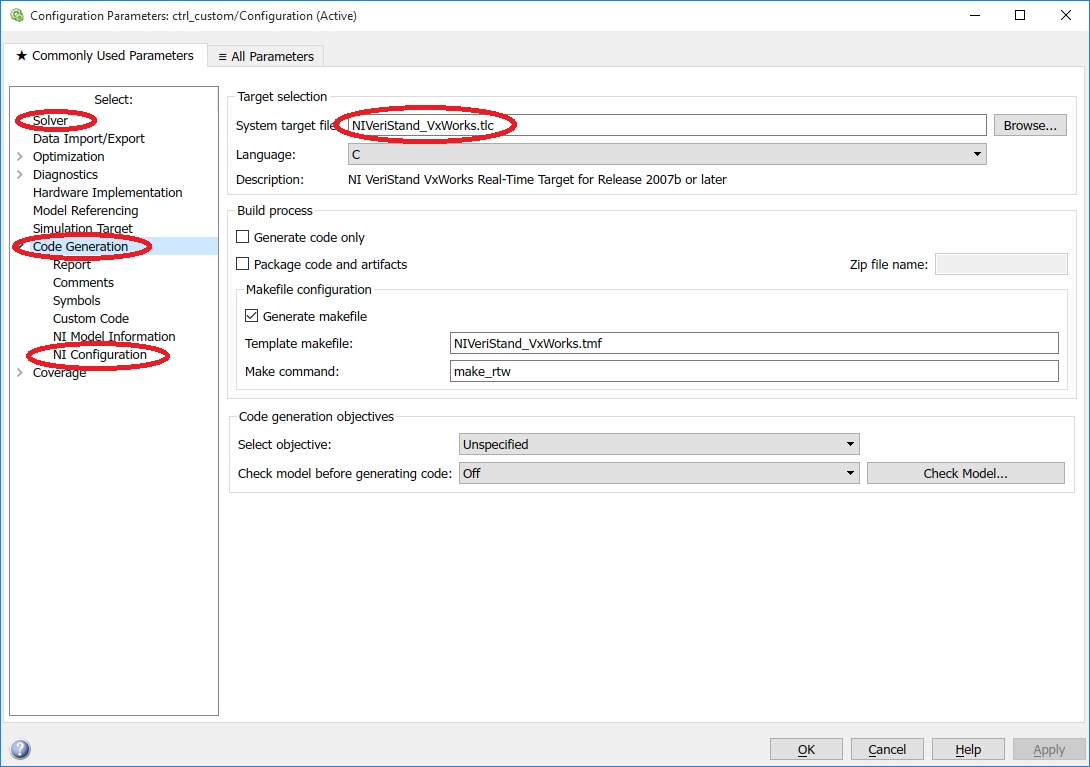
\includegraphics[scale=0.5]{fig/model_conf_window.png}}
		\caption{Model Configuration window}
		\label{fig:model_configuration}
	\end{figure}
	You are now ready to compile the code and include it in the VeriStand project:
	\begin{enumerate}
		\item Compile the Simulink model by pressing \texttt{Ctrl+B} or 
\includegraphics{fig/build.png} in the Simulink window. MATLAB is now compiling your code, and it will update the folder \path{CSE1\Simulink system\ctrl_custom_niVeriStand_VxWorks_rtw} with a cRIO compatible simulation model. 
		\item Open the VeriStand project (\textit{CSE1.nivsproj}), and then open the System Explorer as illustrated in Figure \ref{fig:project_explorer}.
		\item Navigate to the \texttt{ctrl\_custom} Simulation Model, verify the modification date/time is correct (time stamp from when you compiled the simulink model) and then press Reload as illustrated in Figure \ref{fig:system_explorer}. 
		\item Save and close the System Explorer window. 
	\end{enumerate}
	Your Simulink model is now updated and included in the VeriStand project. Continue with preparing the vessel and uploading the code to the cRIO, as described in the vessel specific Handbook. 
	\begin{figure}[htb!]
		\centering
		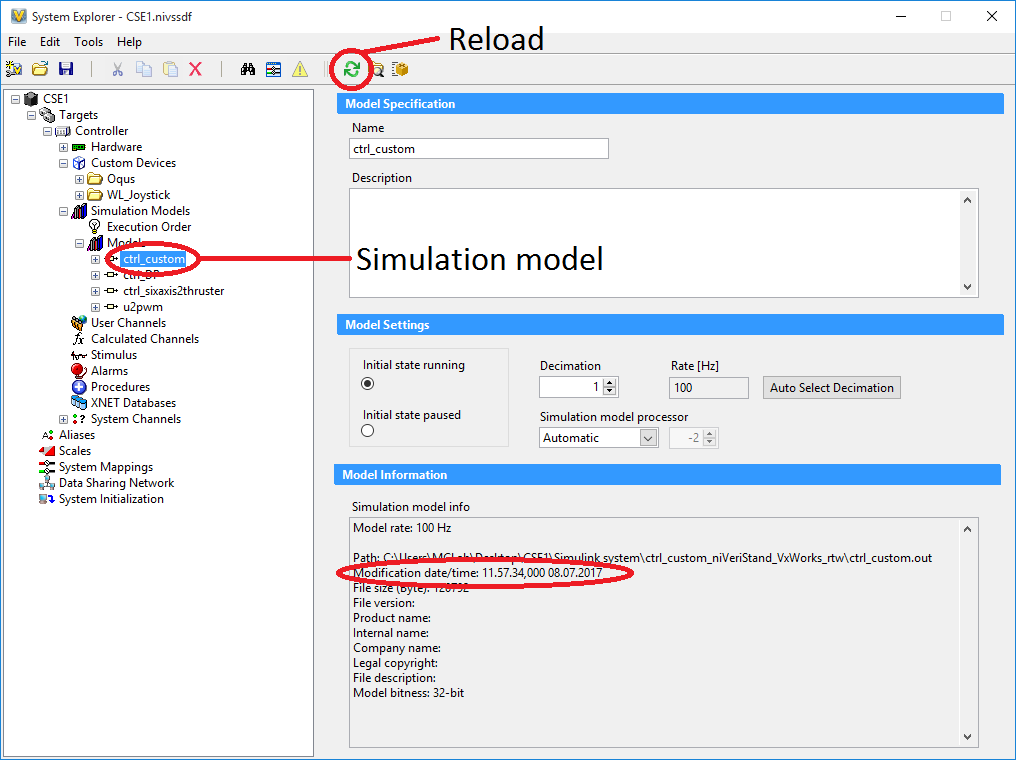
\includegraphics[scale=0.5]{fig/system_explorer.png}
		\caption{System Explorer window}
		\label{fig:system_explorer}
	\end{figure}
\section{Data logging on cRIO}
Logging of data can be done in 2 ways:
\subsection{In Workspace}
Logging channels/parameters from Workspace is done with a Data Logging Controller, found in Workspace Controls. This is the preferred method, as you set the start and stop of data logging and avoid problems if the code does not deploy correctly. The data log is also saved on the laptop, not on the cRIO. Add a Data Logging Control in your Workspace window, set the desired path for the file and add the channels/parameters of interest. See Figure \ref{fig:data_logging}. 
\begin{figure}[htb!]
	\centerline{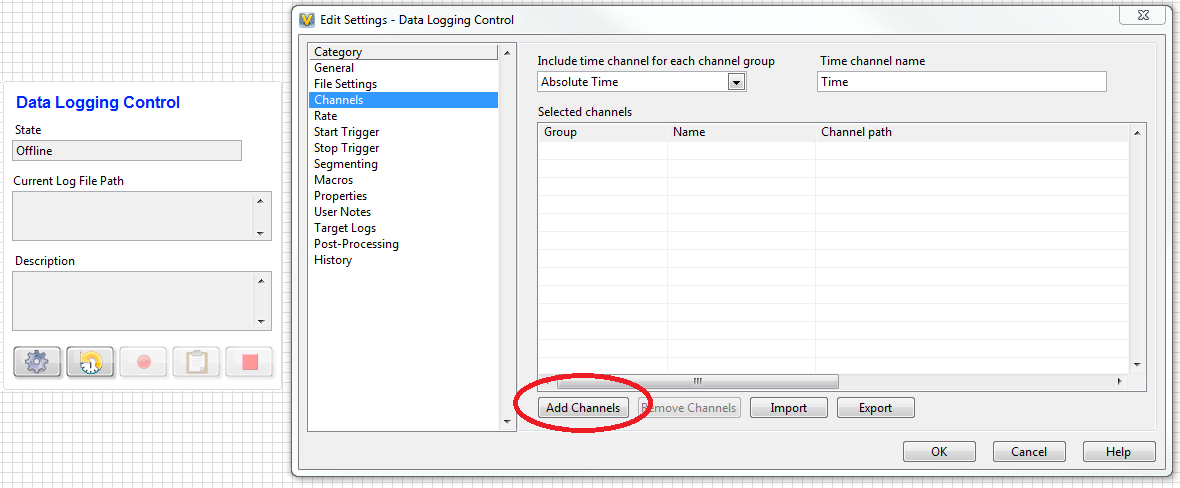
\includegraphics[scale=0.5]{fig/data_logging.png}}
	\caption{Data logging in Workspace}
	\label{fig:data_logging}
\end{figure}
\subsection{In Simulink}
In the Simulink model, it is possible to add "Write to File" blocks linked to the different parameters. By using this method, the cRIO logs the parameters continuously after deployment, until the VeriStand project is undeployed. The data is logged as binary numbers, and if the code is not undeployed correctly(e.g. some error/loss of power etc.), the data log becomes corrupted. However, if this method still is chosen, the data files must be copied from the cRIO to the laptop. Open NI MAX, in the left pane, browse to CSE1, right click on it and choose File Transfer. Copy the logged files to the laptop, which can then be loaded in MATLAB. 
\clearpage
\bibliographystyle{elsarticle-harv}
\bibliography{referencesl}
\appendix
\chapter{Advanced software topics}
\section{Creating FPGA and XML files}
\subsection{Create FPGA target and XML}\label{subsec:Create-FPGA-target}
If you do not have a Veristand FPGA target at your disposal, follow the steps below. If you have a target available and just need to install it in NI Veristand, please jump to Section \ref{sec:install_FPGA_in_veristand}. For CS Enterprise 1 and CS Arctic Drill Ship, the FPGA targets are found on GitHub. 
\begin{enumerate}
	\item Open LabVIEW and create new project. In this guide, LabVIEW 2013 is used, but the procedure should be similar on newer versions. 
	\item Choose NI Veristand FPGA Project in project templates and proceed.
	\item Choose CompactRIO Reconfiguarble Embedded System and click next.
	\item You will now get the choice between letting LabVIEW detect your cRIO  system or configure it yourself. If you are connected to the cRIO and it has all of the I/O ports connected, the option ``Discover existing system'' is simpler and therefore recommneded. If you do not have your cRIO connected choose ``Create new system'', this is the version that will be worked through here.
	\item Select your controller, in our case cRIO-9024.
	\item Select your FPGA target, in our case cRIO-9113.
	\item Then you select your I/O modules to the correct slots. In our case NI 9215 in slot 1 and NI 9474 in slot 4.
	\item You are now finished with configuring your project. Press next.
	\item The project menu will now appear and should look something like Figure
	\ref{fig: Create Labview FPGA target and XML-10}. Select the LabVIEW VI as demonstrated our is called Custom Personality FPGA.vi
	\item The UI window will now present itself, select window and show block diagram.
	\item You should now see a block diagram similar to Figure \ref{fig: Create Labview FPGA target and XML-11}. You will now have to redesign this to look like Figure \ref{fig: Create Labview FPGA target and XML-12}. This will be valid for our system, if you have different I/O modules the block diagram need to reflect this.
	\item Now, return to the Project explorer and select Build Specifications and Custom Personality FPGA
	\item A new window will open. Check that the name and project path is correct and press build.
	\item Select your preferred compile server. The compilation process will take quite some time (approx 15-30 min).
	\item When the compilation process is finished, the last step is to edit the automatically generated XML file. You will now have to find you project directory in Windows. Here there will be a folder called bitfiles which contains the files you compiled in the last step, there will also be a .XML file. The point of editing this file is to match the actually compiled VI, meaning the packets must match the connected I/O. The recommended way to edit the file is to copy our XML file from: Dropbox\textbackslash{}TMR4243 - LAB\textbackslash{}04 cRIO software\textbackslash{}FPGA IO. You will have to make sure that the name of your bitfile matches the name in the XML file as seen in Figure \ref{fig: Create Labview FPGA target and XML-17}, also make sure the I/O modules matches your setup.
	\item Copy the bitfiles from the bitfile folder to the level above so that the bitfile aand the XML file is in the same folder.
\end{enumerate}
Documentation: \url{https://decibel.ni.com/content/docs/DOC-13815}

\begin{figure}[htb!]
	\centering 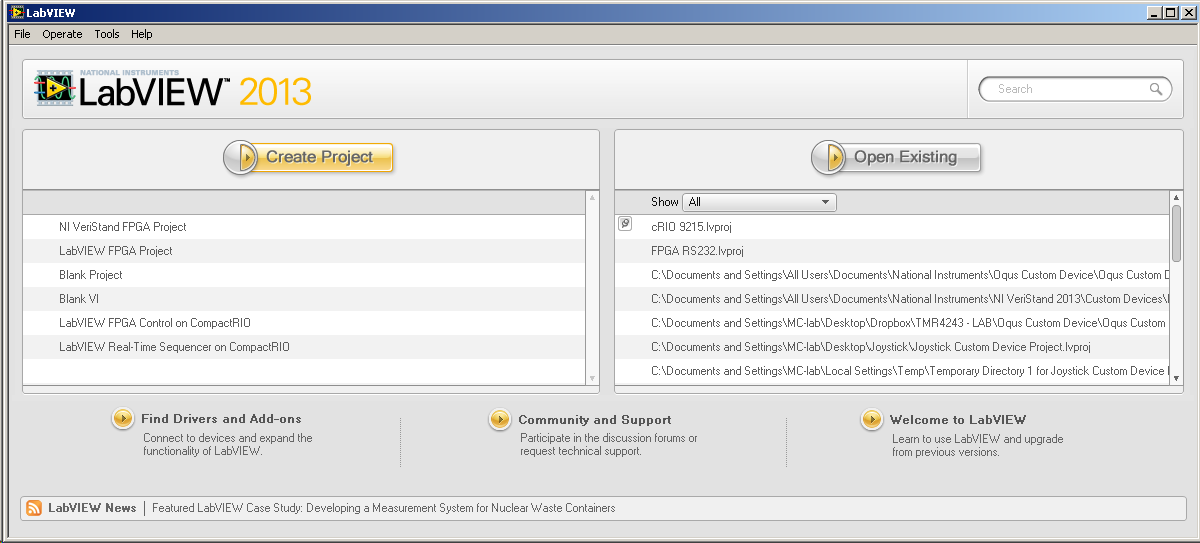
\includegraphics[scale=0.45]{Screenshots/Screenshot_2015-01-16_19-21-16.png}
	\caption{Create Labview FPGA target and XML - 1}
	\label{fig: Create Labview FPGA target and XML-1} 
\end{figure}
\begin{figure}[htb!]
	\centering 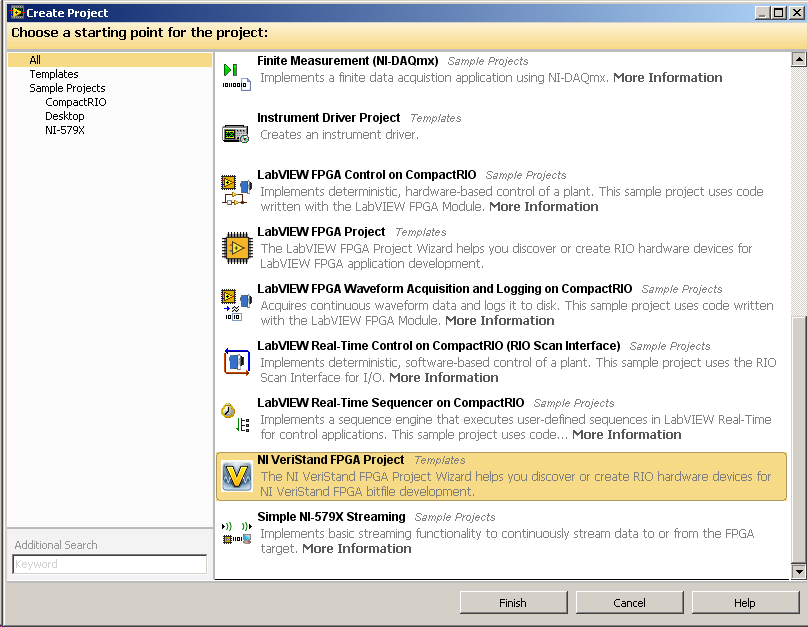
\includegraphics[scale=0.45]{Screenshots/Screenshot_2015-01-16_19-23-23.png}
	\caption{Create Labview FPGA target and XML - 2}
	\label{fig: Create Labview FPGA target and XML-2} 
\end{figure}
\begin{figure}[htb!]
	\centering 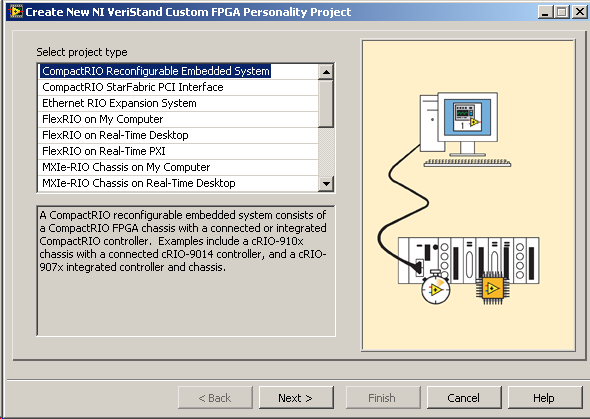
\includegraphics[scale=0.45]{Screenshots/Screenshot_2015-01-16_19-23-41.png}
	\caption{Create Labview FPGA target and XML - 3}
	\label{fig: Create Labview FPGA target and XML-3} 
\end{figure}
\begin{figure}[htb!]
	\centering 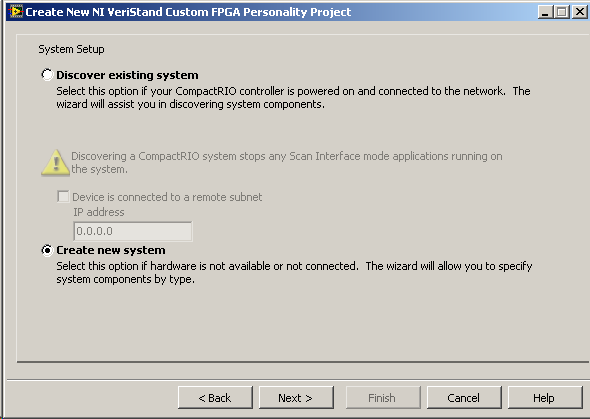
\includegraphics[scale=0.45]{Screenshots/Screenshot_2015-01-16_19-23-58.png}
	\caption{Create Labview FPGA target and XML -4}
	\label{fig: Create Labview FPGA target and XML-4} 
\end{figure}
\begin{figure}[htb!]
	\centering 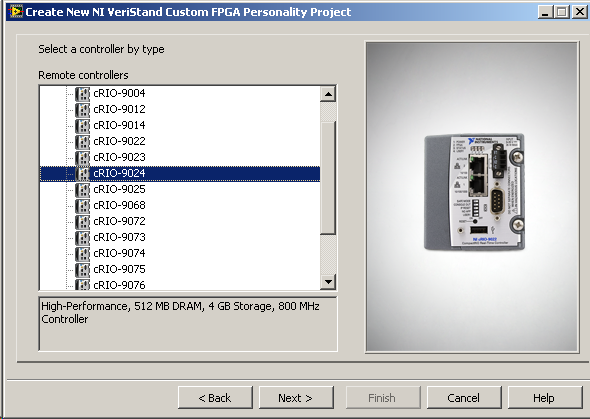
\includegraphics[scale=0.45]{Screenshots/Screenshot_2015-01-16_19-24-31.png}
	\caption{Create Labview FPGA target and XML - 5}
	\label{fig: Create Labview FPGA target and XML-5} 
\end{figure}
\begin{figure}[htb!]
	\centering 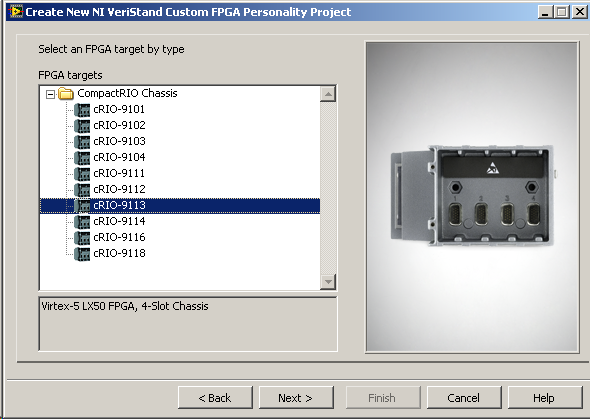
\includegraphics[scale=0.45]{Screenshots/Screenshot_2015-01-16_19-24-43.png}
	\caption{Create Labview FPGA target and XML - 6}
	\label{fig: Create Labview FPGA target and XML-6} 
\end{figure}
\begin{figure}[htb!]
	\centering 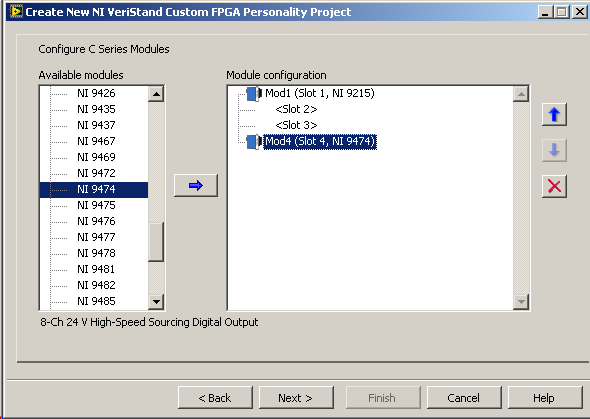
\includegraphics[scale=0.45]{Screenshots/Screenshot_2015-01-16_19-25-37.png}
	\caption{Create Labview FPGA target and XML - 7}
	\label{fig: Create Labview FPGA target and XML-7} 
\end{figure}
\begin{figure}[htb!]
	\centering 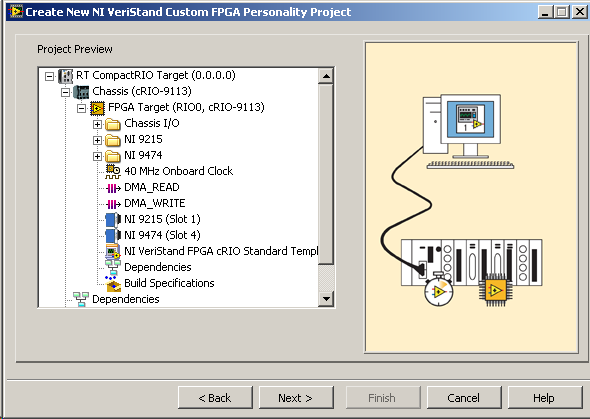
\includegraphics[scale=0.45]{Screenshots/Screenshot_2015-01-16_19-25-54.png}
	\caption{Create Labview FPGA target and XML - 8}
	\label{fig: Create Labview FPGA target and XML-8} 
\end{figure}
\begin{figure}[htb!]
	\centering 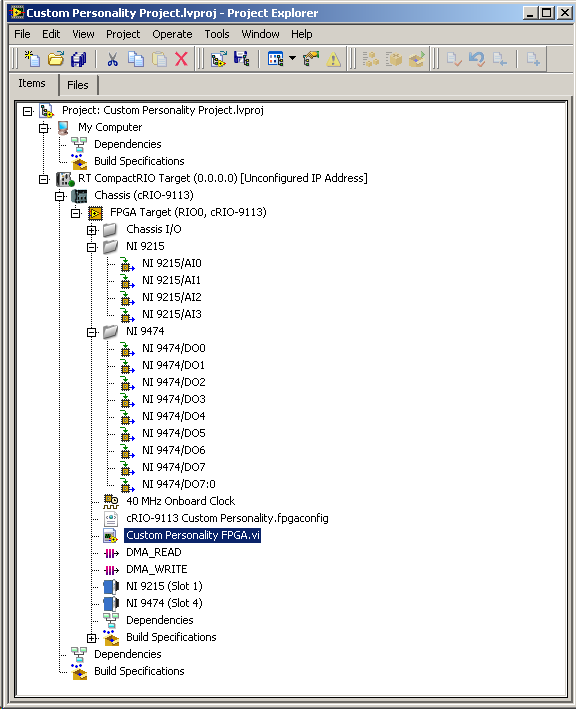
\includegraphics[scale=0.45]{Screenshots/Screenshot_2015-01-16_19-28-17.png}
	\caption{Create Labview FPGA target and XML -9}
	\label{fig: Create Labview FPGA target and XML-9} 
\end{figure}
\begin{figure}[htb!]
	\centering 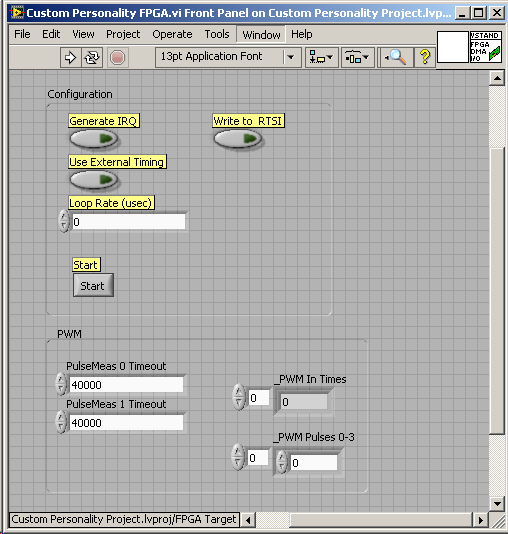
\includegraphics[scale=0.45]{Screenshots/Screenshot_2015-01-16_19-28-41.png}
	\caption{Create Labview FPGA target and XML - 10}
	\label{fig: Create Labview FPGA target and XML-10} 
\end{figure}
\begin{figure}[htb!]
	\centering 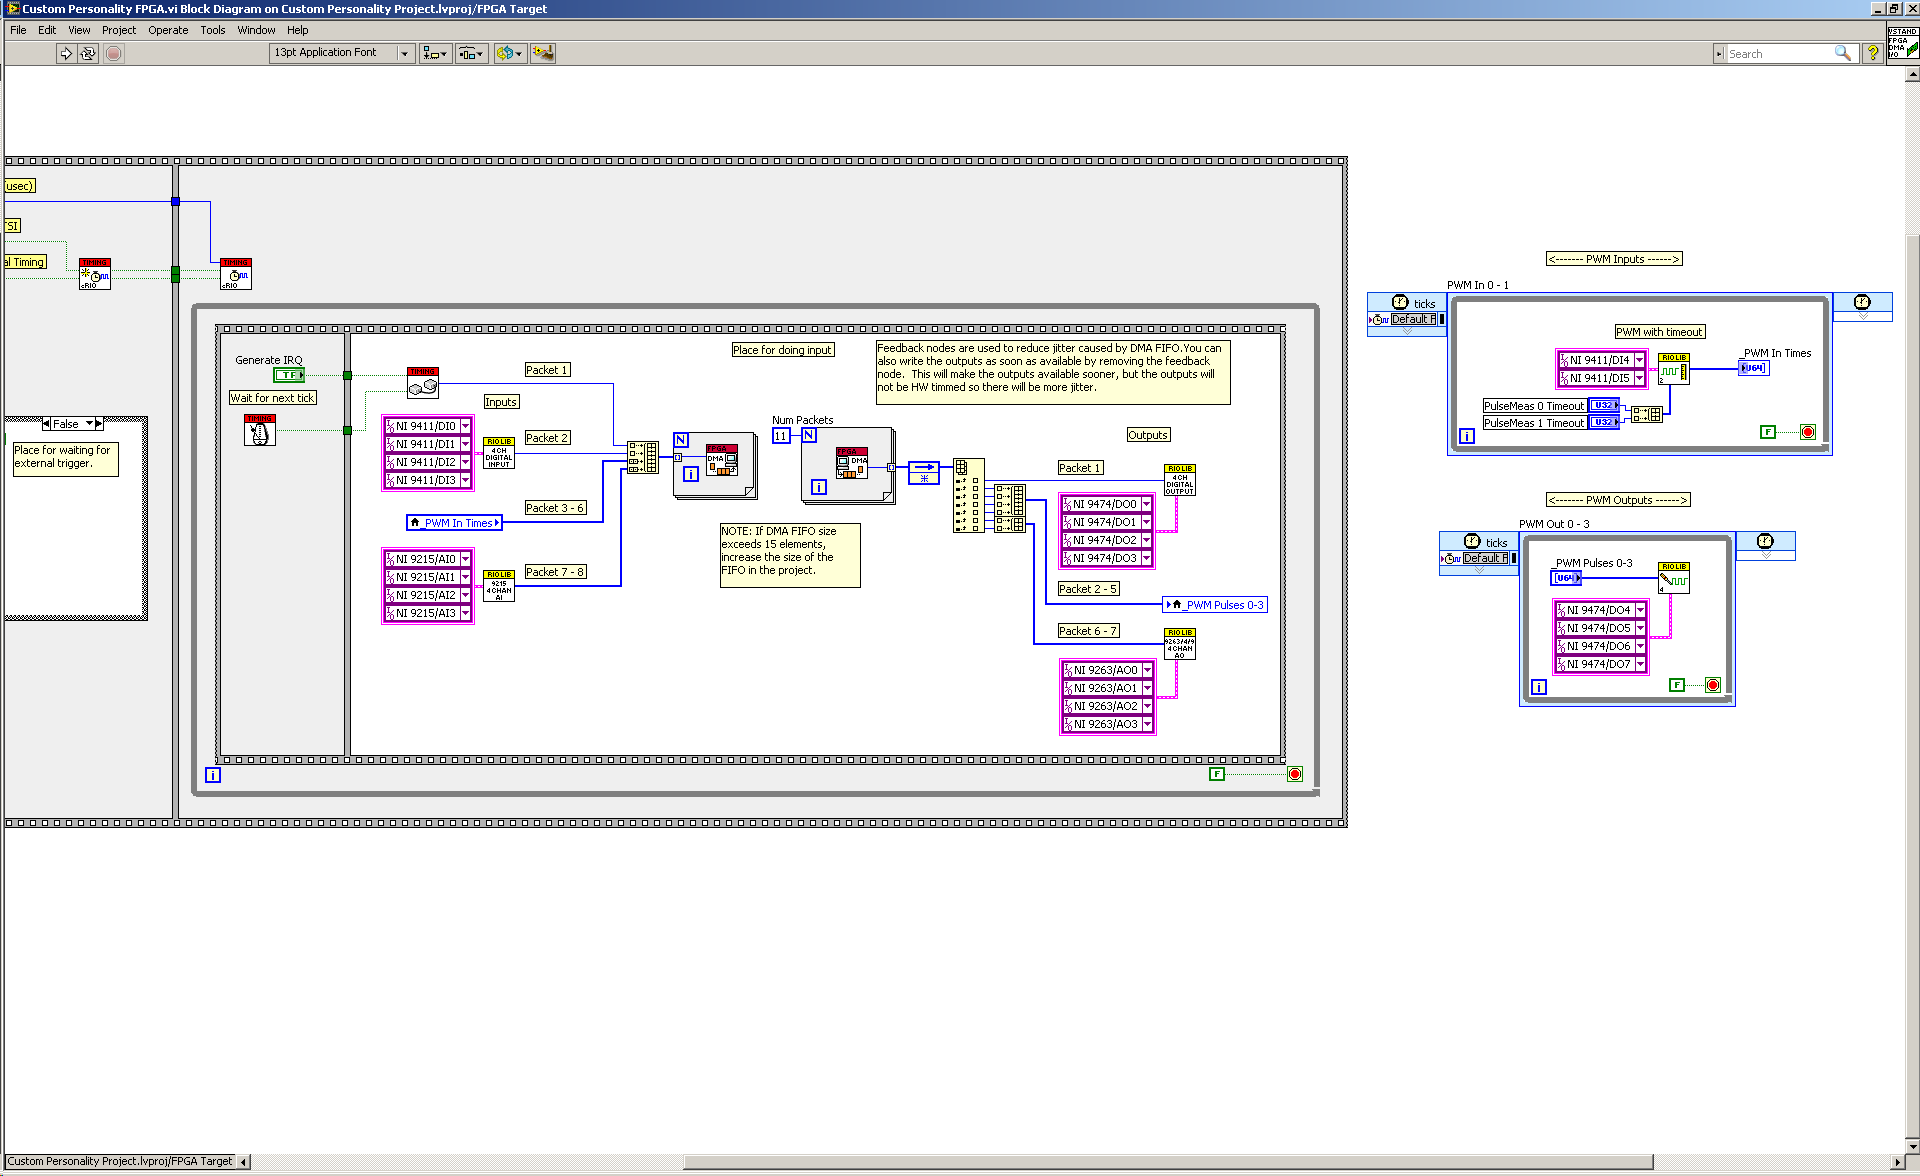
\includegraphics[angle=-90,scale=0.45]{Screenshots/Screenshot_2015-01-16_19-29-04.png}
	\caption{Create Labview FPGA target and XML - 11}
	\label{fig: Create Labview FPGA target and XML-11} 
\end{figure}
\begin{figure}[htb!]
	\centering 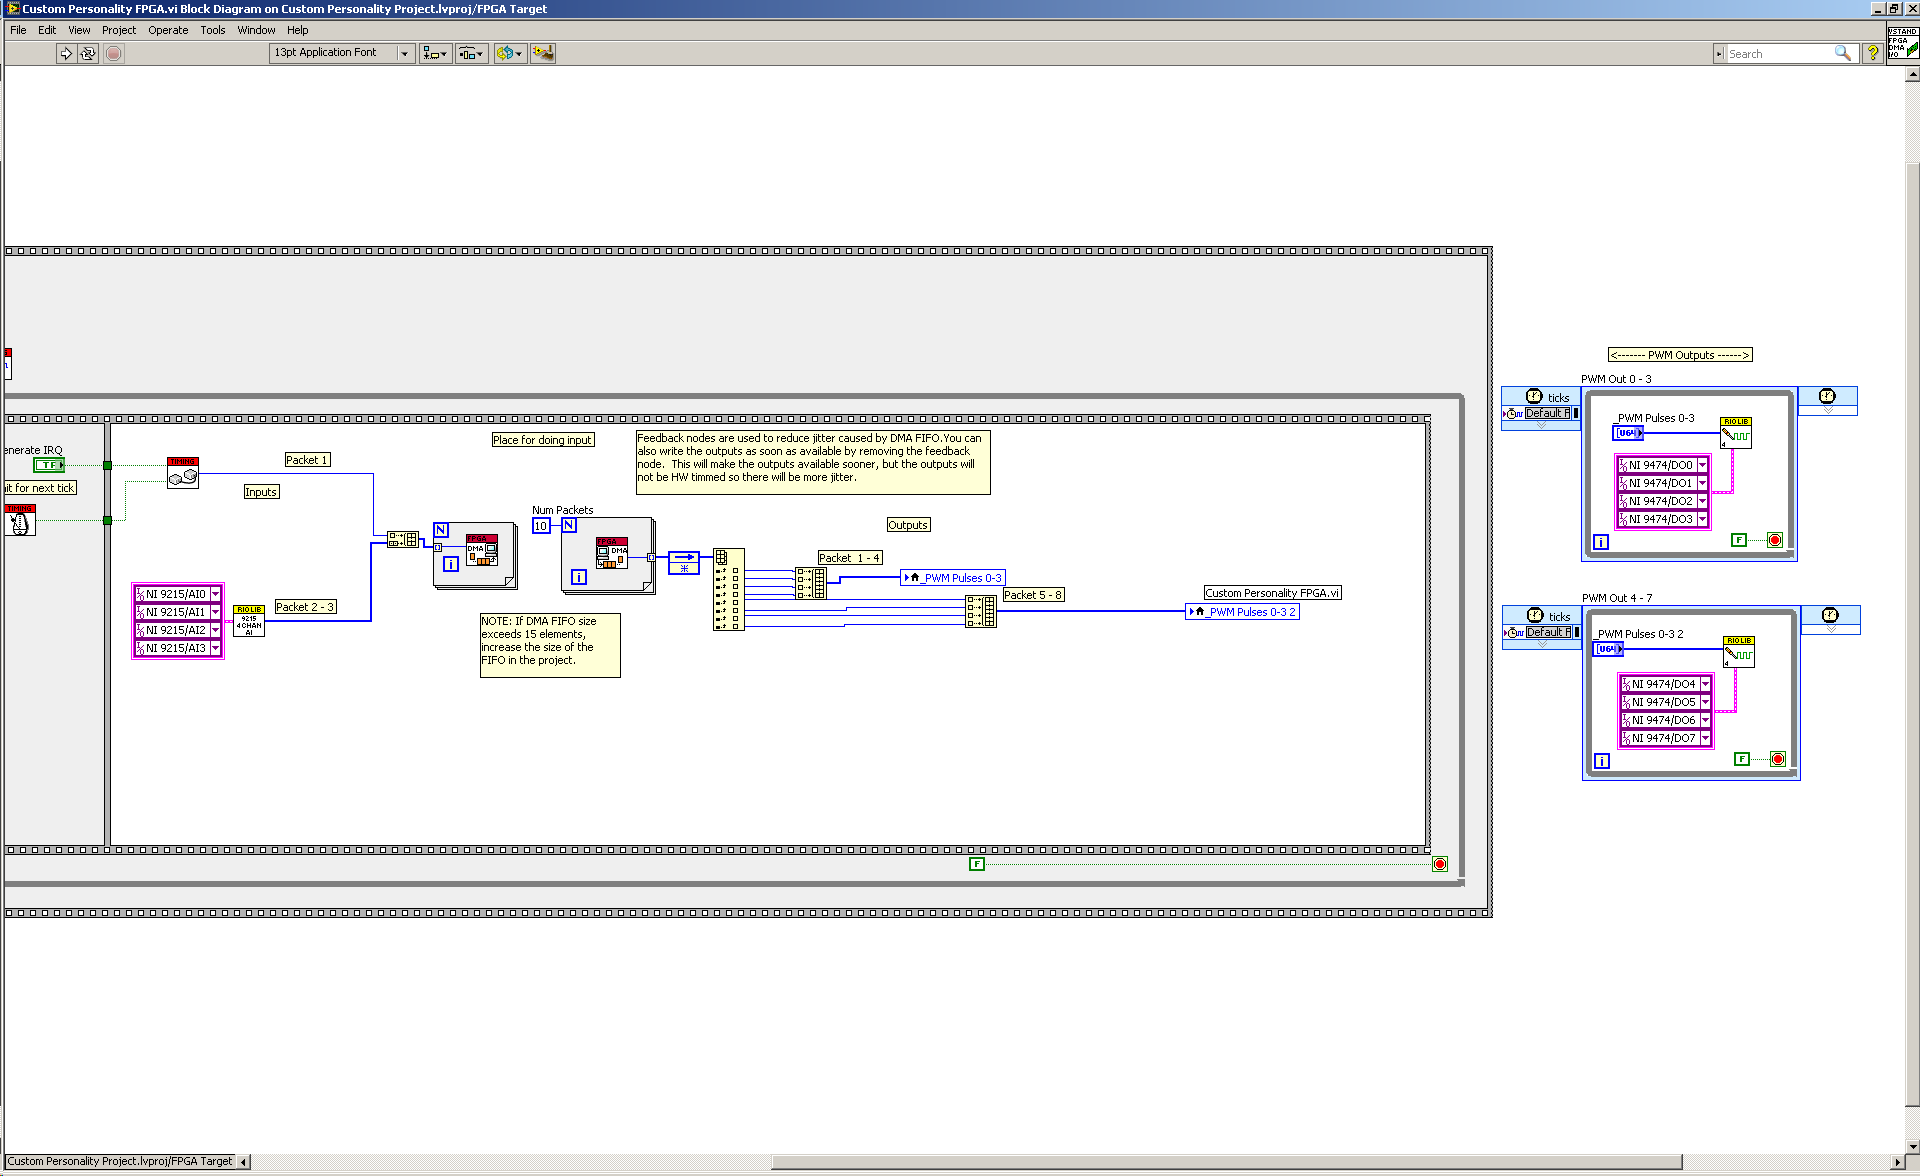
\includegraphics[angle=-90,scale=0.45]{Screenshots/Screenshot_2015-01-16_20-07-43.png}
	\caption{Create Labview FPGA target and XML - 12}
	\label{fig: Create Labview FPGA target and XML-12} 
\end{figure}
\begin{figure}[htb!]
	\centering 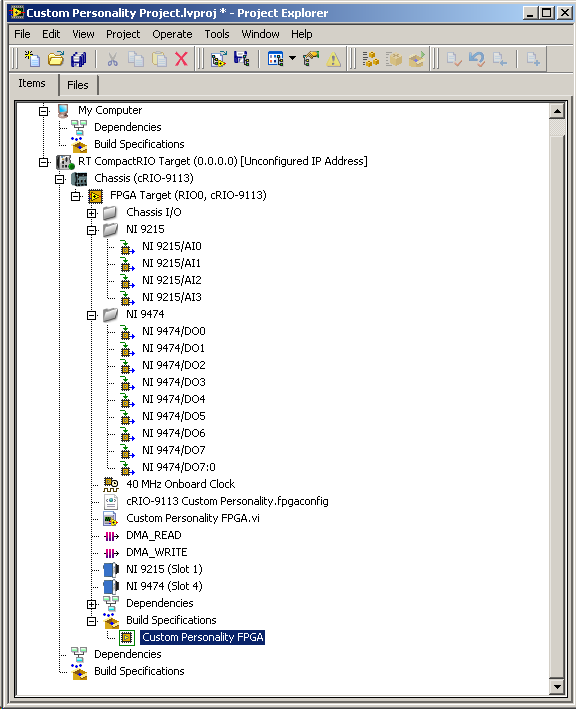
\includegraphics[scale=0.45]{Screenshots/Screenshot_2015-01-16_19-52-25.png}
	\caption{Create Labview FPGA target and XML - 13}
	\label{fig: Create Labview FPGA target and XML-13} 
\end{figure}
\begin{figure}[htb!]
	\centering 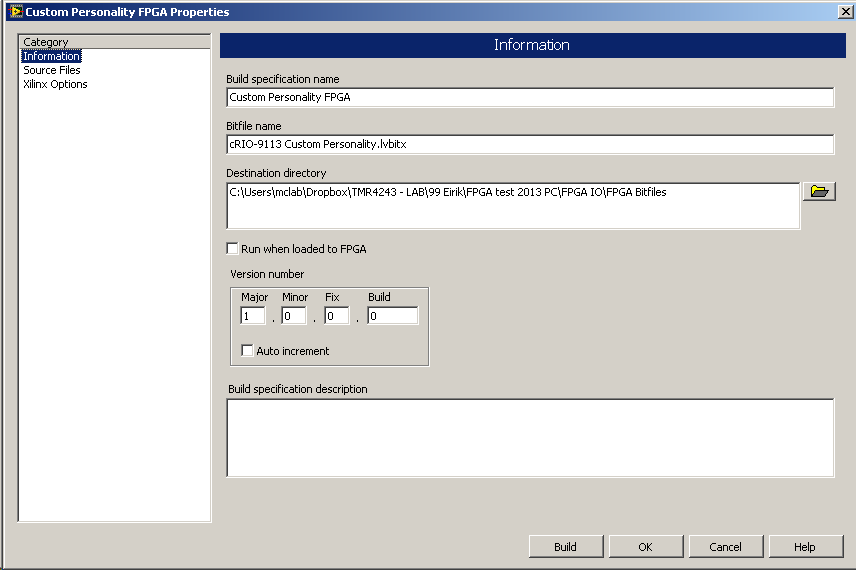
\includegraphics[scale=0.45]{Screenshots/Screenshot_2015-01-16_19-53-01.png}
	\caption{Create Labview FPGA target and XML - 14}
	\label{fig: Create Labview FPGA target and XML-14} 
\end{figure}
\begin{figure}[htb!]
	\centering 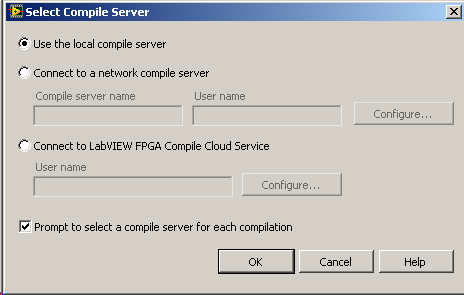
\includegraphics[scale=0.45]{Screenshots/Screenshot_2015-01-16_19-53-25.png}
	\caption{Create Labview FPGA target and XML - 15}
	\label{fig: Create Labview FPGA target and XML-15} 
\end{figure}
\begin{figure}[htb!]
	\centering 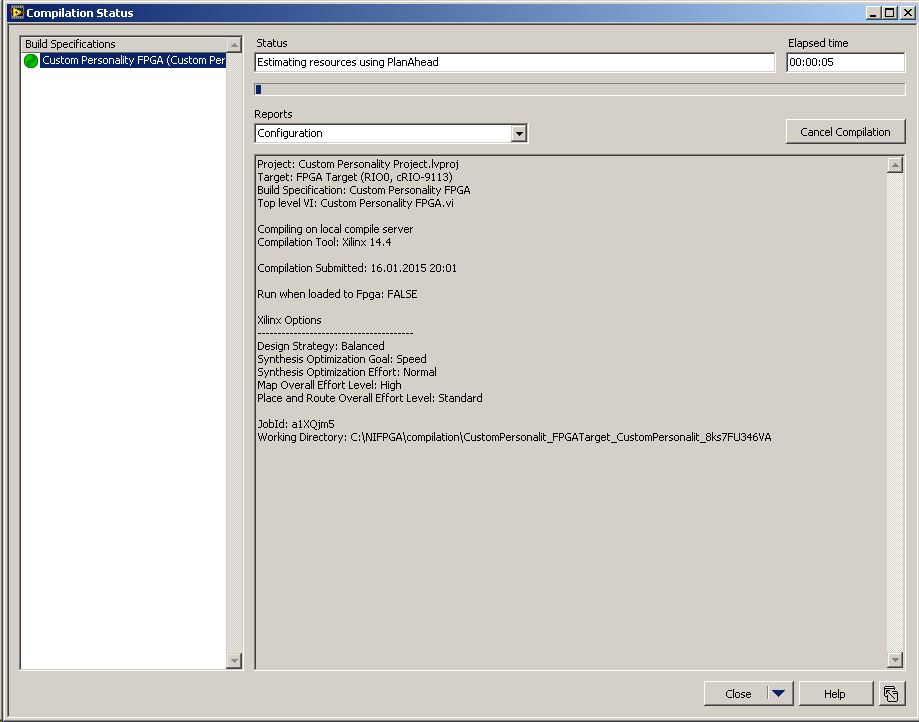
\includegraphics[scale=0.45]{Screenshots/Screenshot_2015-01-16_20-01-32.png}
	\caption{Create Labview FPGA target and XML - 16}
	\label{fig: Create Labview FPGA target and XML-16} 
\end{figure}
\begin{figure}[htb!]
	\centering 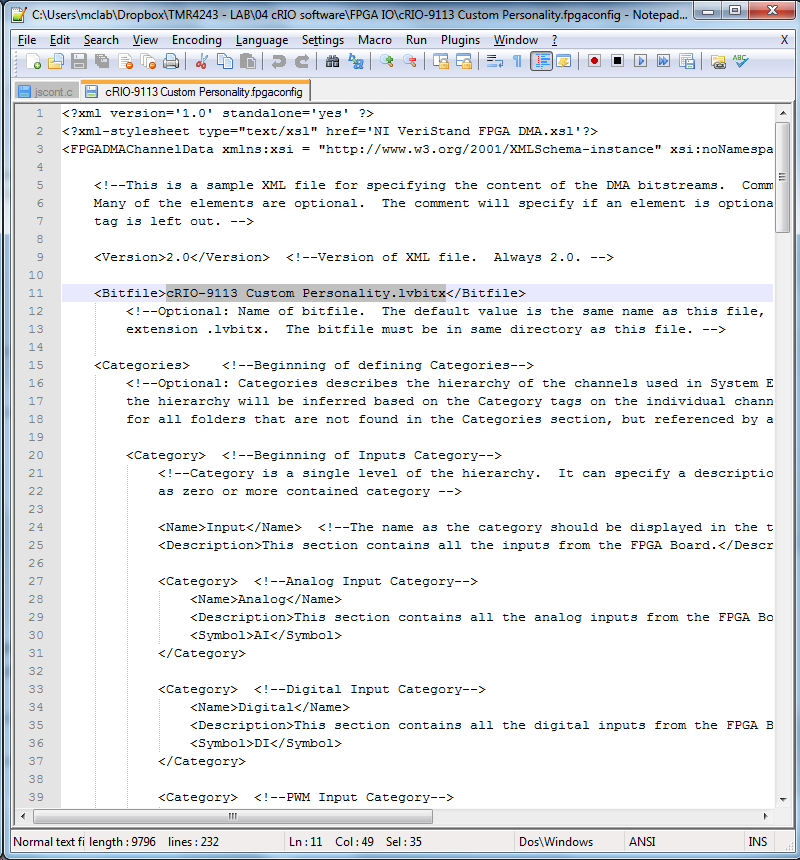
\includegraphics[scale=0.45]{Screenshots/Screenshot_2015-01-17_13-59-31.png}
	\caption{Create Labview FPGA target and XML - 17}
	\label{fig: Create Labview FPGA target and XML-17} 
\end{figure}

\subsection{Install in VeriStand}\label{sec:install_FPGA_in_veristand}

The Veristand software does not recognize the physical I/O components of the cRIO. It is necessarry to write a specific FPGA mapping for the specific setup. This results in a XML file that maps the ports. 

To add this file to your Veristand project, enter the system explorer and find the FPGA pane under \textit{targets\textbackslash{}controller\textbackslash{}hardware\textbackslash{}chassis}, as seen in Figure \ref{fig: fpga1}. 
\begin{figure}[htb!]
	\centering 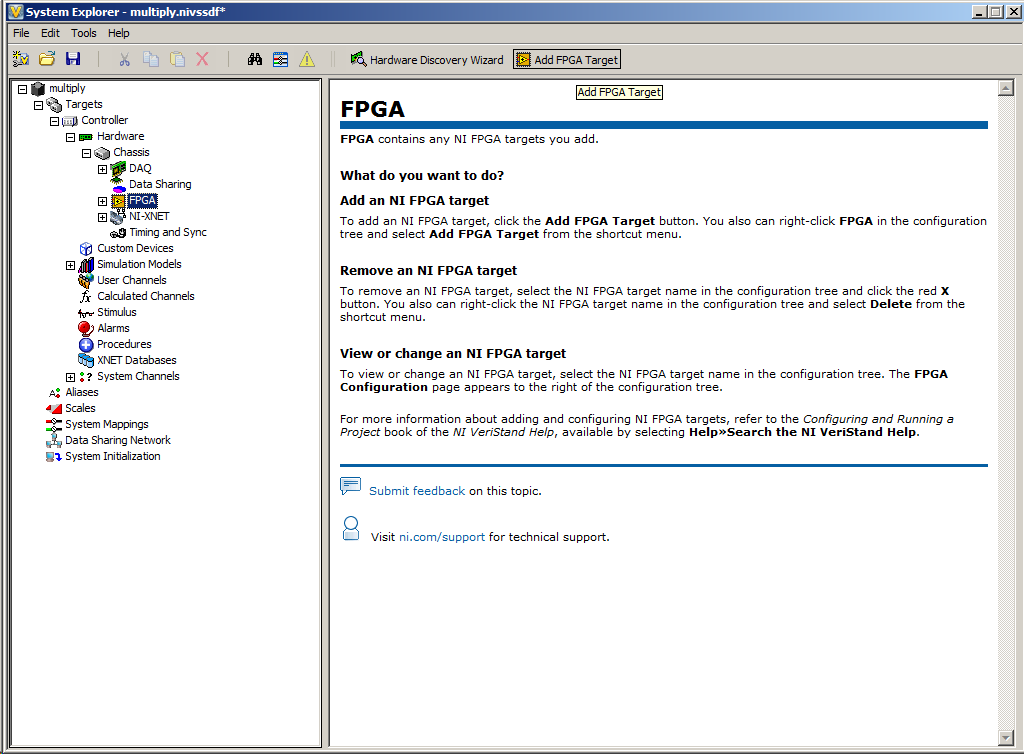
\includegraphics[scale=0.45]{fig/fpga1}
	\caption{FPGA1}
	\label{fig: fpga1}
\end{figure}
The next step is to find your XML file. In this case called cRIO-9113 Ex, it is very important that the XML file is placed on level above the FPGA bitfile folder in the directory system, as the files are really being used are the FPGA bitfiles.
\begin{figure}[htb!]
	\centering 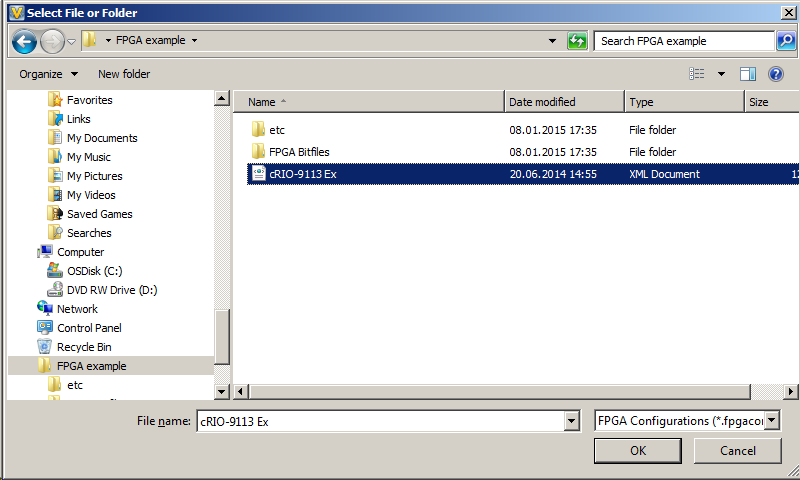
\includegraphics[scale=0.45]{fig/fpga2}
	\caption{FPGA2}
	\label{fig: fpga2}
\end{figure}
The menu in should now look something like Figure \ref{fig: fpga2}, here you can see the analogue input signals and the digital output PWM signals. These can again be linked to other signals as seen in Figure\ref{fig: veristand mappings}.
\begin{figure}
	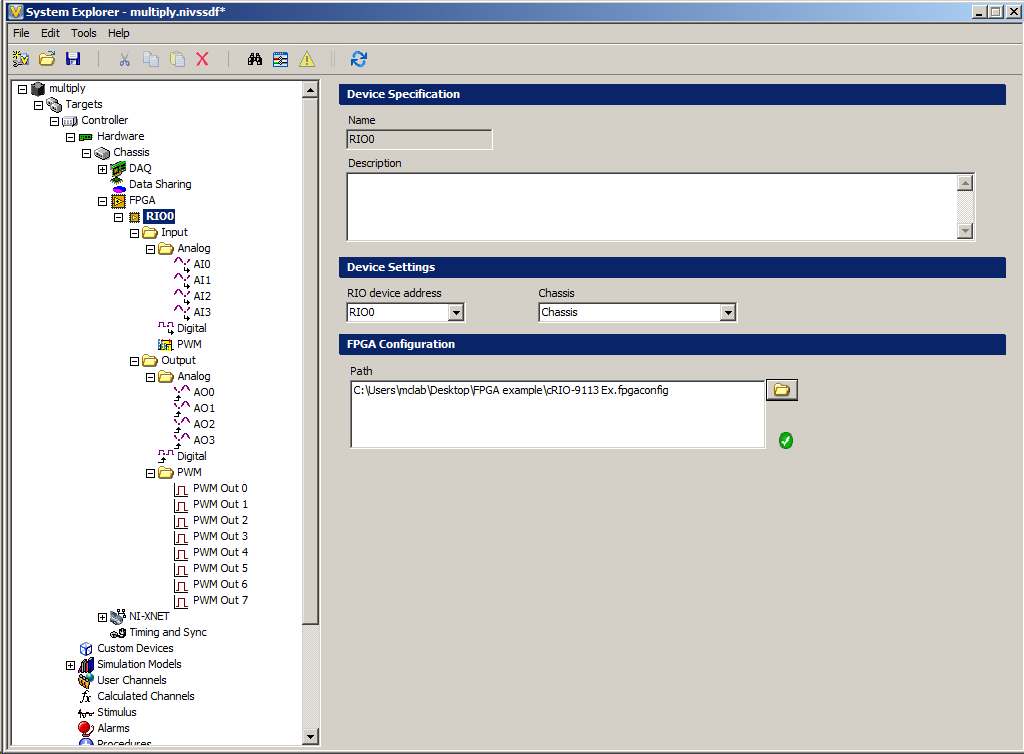
\includegraphics[scale=0.45]{fig/fpga3}
	\caption{FPGA3}
	\label{fig: fpga3}
\end{figure}
\subsubsection{Ticks}
tick = FPGA clock pulse
\[\text{tick in seconds}=\frac{1}{\text{frequency}}=\frac{1}{40MHz}=\frac{1}{40*10^{6}}=25*10^{-}9=25ns\]
output at 50 Hz demands output every 
\[\frac{40MHz}{50Hz}=\frac{40*10^{6}}{50}=800000tick\]
\section{Custom Device}
\subsection{Install}\label{subsec: Installing custom device driver}
As of July 2017, there are 3 different Custom Device drivers developed for use in MCLab: 
\begin{description}
	\item [WL\_Joystick] - used for reading sixaxis data sent from the RPi. Created by Torgeir Wahl
	\item [Oqus] - used for reading position and orientation data sent from the Qualisys system. Created by Torgeir Wahl
	\item [IMU] - used for reading IMU data from 4 IMU's, mainly intended for CSAD. Created by Guttorm Udjus
\end{description}
To install a Custom Device driver, the first step is to copy the folder with the driver to the path: \path{C:\Users\Public\Documents\National Instruments\NI VeriStand 201X\Custom Devices}
The directory should now contain something like Figure \ref{fig: custom device folder}.
\begin{figure}[htb!]
	\centering 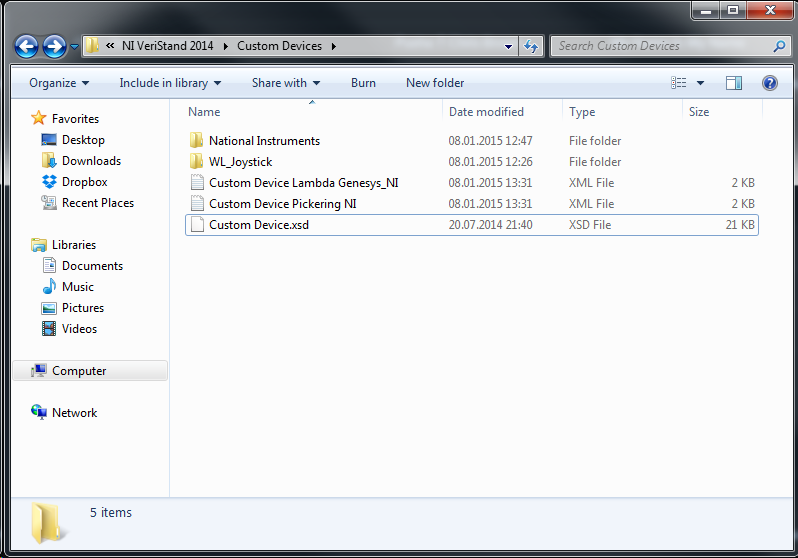
\includegraphics[scale=0.45]{fig/custom_devices_folder.png}
	\caption{Custom device folder}
	\label{fig: custom device folder} 
\end{figure}
The next step is to add custom device to your project. This is done in the system explorer, which is found as seen in Figure \ref{fig: veristand launch system explorer}.
\begin{figure}[htb!]
	\centering \includegraphics[scale=0.45]{fig/"veristand launch system explorer".png}
	\caption{VeriStand launch system explorer}
	\label{fig: veristand launch system explorer} 
\end{figure}
When in the system explorer, adding the custom device should be as simple as right clicking the custom device pane and choosing WL\_Joystick, as in Figure \ref{fig: custom device selection}. If you do not find the custom device WL\_Joystick, the most likely problem is that the placement of the custom device folder from step 1 is wrong.
\begin{figure}[htb!]
	\centering \includegraphics[scale=0.45]{fig/"veristand custom driver select".png}
	\caption{Custom device selection}
	\label{fig: custom device selection} 
\end{figure}
If the installation is successful you should be able to see WL\_Joystick folder under custom devices as seen in the red box in Figure \ref{fig: veristand confirmation}. Here you will also see the different inputs from the custom device, in this case it is joystick axis.
\begin{figure}[htb!]
	\centering \includegraphics[scale=0.45]{fig/"veristand mapping".png}
	\caption{VeriStand}
	\label{fig: veristand confirmation} 
\end{figure}
To connect the joystick to the input ports of the Simulink model. You open the system configuration mappings (click the button marked by the arrow in Figure \ref{fig: veristand confirmation}).
\begin{figure}[htb!]
	\centering \includegraphics[scale=0.45]{fig/"veristand mapping2".png}
	\caption{VeriStand System Configuration Mappings}
	\label{fig: veristand mappings} 
\end{figure}
You the simply find the ports you would like to connect, mark them and click the connect button. Figure \ref{fig: veristand mappings} a joystick output is connected to a input port on the Simulink model.
\section{Raspberry Pi}\label{subsec: RPi setup}
The unit is configured with Raspbian Linux-kernel-based operating system 
\subsection{Raspbian installation and setup}
This section describes how to install and access the Raspbian operating system on the RPi from a Windows computer. The operations are also possible from an OSX or Linux computer.
\subsubsection{Download operating system and utilities}
Download and extract the newest Raspbian\footnote{raspberrypi.org/downloads} operating system (OS) image. Necessary utilities for the setup are
\begin{itemize}
	\item Win32 Disk Imager\footnote{sourceforge.net/projects/win32diskimager} to write the OS image to the RPi SD card
	\item Advanced IP scanner\footnote{by Famatech, advanced-ip-scanner.com} to find the RPi address on the network 
	\item Putty terminal emulator\footnote{www.chiark.greenend.org.uk/\textasciitilde{}sgtatham/putty/download.html} for SSH connection
	\item WinSCP\footnote{by Martin Prikryl, winscp.net/eng/download.php} for file transfer
\end{itemize}
\begin{table}[h!]
	\centering
	\begin{tabular}{ll}
		\hline
		Windows & Linux, OSX\\
		\hline 
		Win32 Disk Imager & dd\\
		Advanced IP scanner & nmap\\
		Putty & ssh\\
		WinSCP & sftp\\
		\hline
	\end{tabular}
	\caption{RPi installation and setup utilities}
	\label{tab:RPi_utilities} 
\end{table}
See Table \ref{tab:RPi_utilities} for a list of the equivalent software for OSX and Linux.
\subsubsection{Write image to SD card}
Since the .iso file is raw, it needs to be written to the SD card in way that makes it bootable. Win32 Disk Imager does this.
\begin{figure}[htb!]
	\centering \includegraphics[scale=0.45]{fig/Rpi_DiskImager} \caption{Disk Imager}
	\label{fig: Disk Imager} 
\end{figure}
Run the program as administrator. Select the correct image file and device, as in Figure \ref{fig: Disk Imager}. Make sure that you have selected the correct drive before you push \texttt{Write}. Once the write is complete, insert the SD card in the RPi and boot.
\subsubsection{Terminal access}\label{subsec: Terminal access}
RPi can be accessed through the network, i.e. without having to directly connect a monitor and keyboard.
\begin{figure}[htb!]
	\centering \includegraphics[scale=0.45]{fig/advancedIPscanner} \caption{Advanced IP Scanner}
	\label{fig: Advanced IP Scanner} 
\end{figure} 
At first boot, the RPi by default waits to be assigned an IP address by DHCP. If this address is not known, scan the network with Advanced IP Scanner. It is advicible to sort the results by manufacturer since it is fixed (\textit{Raspberry Pi Foundation}). The name is typically \emph{raspberrypi}. See Figure \ref{fig: Advanced IP Scanner}.
\begin{figure}[htb!]
	\centering \includegraphics[scale=0.45]{fig/Rpi_remote_access1} \caption{Putty settings}
	\label{fig: Putty settings} 
\end{figure}
Once the IP is known, it is specified in the Putty settings, as in Figure \ref{fig: Putty settings}, and a connection can be opened. 
\begin{figure}[htb!]
	\centering \includegraphics[scale=0.45]{fig/Rpi_remote_access2} \caption{SSH connection}
	\label{fig: SSH connection} 
\end{figure}
The default login is \texttt{pi}, and the default password \texttt{raspberry}. Figure \ref{fig: SSH connection} shows the terminal output on first login.
\subsubsection{Finalize configuration}
\begin{figure}[htb!]
	\centering 
	\includegraphics[scale=0.45]{fig/Rpi_finalize_install} 
	\caption{RPi configuration tool}
	\label{fig: RPi configuration tool} 
\end{figure}
Enter the\begin{verbatim}sudo raspi-config\end{verbatim}command to start the RPi Software Configuration Tool, as in Figure \ref{fig: RPi configuration tool}. Use the menu to apply the following
\begin{enumerate}
	\item Update configuration tool: 8 Advanced Options \textgreater  A9 Update
	\item Change password: 2 Change User Password
	\item Expand filesystem: 1 Expand Filesystem \textgreater  Finish
\end{enumerate}
Exit the configuration tool and select \texttt{Yes} for reboot. Reconnect through Putty.
Finally, update the repository package lists and upgrade all packages currently installed on the RPi:\begin{verbatim}sudo apt-get update 
sudo apt-get upgrade -y\end{verbatim}This process took approximately 10 minutes on a 90 Mbps internet connection. 
\subsubsection{Transfer files to RPi from computer}\label{subsec: Transfer files to RPi}
WinSCP can be used to transfer files to the RPi. This is useful for instance when transferring code, or when the RPi is not directly connected to the internet.
\subsubsection{Set fixed IP address}
When the RPi is connected directly to the cRIO or computer, a fixed IP is necessary since there is no DHCP server in that network. During most of this setup, however, it is preferable to keep the default DHCP assigned IP setting. To set a fixed IP
\begin{enumerate}
	\item Open the network interface configuration information file for editing\begin{verbatim}sudo nano /etc/network/interfaces\end{verbatim}
	\item Alter the eth0 settings from \texttt{dhcp} to \texttt{static} and
	add address and netmask as\begin{verbatim}auto eth0
	iface eth0 inet static
	address 192.168.1.22
	netmask 255.255.255.0\end{verbatim}
	\item Save the changes by the key combination \texttt{Ctrl+X}.
\end{enumerate}
The new IP is applied on the next reboot.

\subsection{Sixaxis installation and configuration}
This section describes how to install and configure the Sixaxis gamepad for Bluetooth connection to the RPi, and how to add a server for sending joystick signals to the cRIO.
\subsubsection{Download and install bluetooth support}
BlueZ is the official Linux Bluetooth stack. It provides support for core Bluetooth layers and protocols. To download and install, type
\begin{verbatim}sudo apt-get install bluez-utils bluez-compat bluez-hcidump
libusb-dev libbluetooth-dev joystick checkinstall -y\end{verbatim}
The process takes a few minutes.
\begin{figure}[htb!]
	\centering \includegraphics[scale=0.45]{fig/rpi_hciconfig} \caption{Bluetooth configuration tool}
	\label{fig: RPi hciconfig} 
\end{figure}
To confirm the installation, use the \texttt{hciconfig} command to print name and basic information about Bluetooth devices installed in the system. The output should include \texttt{UP RUNNING PSCAN}, as in Figure \ref{fig: RPi hciconfig}. If instead it says \texttt{DOWN}, some error har occured. Most experienced errors were due to typos.
\subsubsection{Bluetooth pairing}\label{par: Bluetooth-pairing}
Sixaxis does not support the standard Bluetooth paring prcedure, instead, pairing is done over USB. The \texttt{sixpair} command-line utility\footnote{by Pabr Technologies, www.pabr.org} searches USB buses for Sixaxis devices and tells them to connect to a new Bluetooth master.

Download and compile the program by the following commands:
\begin{verbatim}wget http://www.pabr.org/sixlinux/sixpair.c
gcc -o sixpair sixpair.c -lusb\end{verbatim}
Connect the Sixaxis by USB before running the paring utility
\begin{verbatim}sudo ./sixpair\end{verbatim}
The output should be similar to
\begin{verbatim}Current Bluetooth master: 00:02:72:BF:BC:8F
Setting master bd_addr to: 00:02:72:BF:BC:8F\end{verbatim}
The addresses at the end of each line will only be the same if you have already paired the Sixaxis with the Bluetooth dongle. First time they will be different. The Sixaxis USB cable may now be disconnected.

\subsubsection{Joystick manager system service}
\texttt{QtSixA}\footnote{the Sixaxis Joystick Manager by falkTX, qtsixa.sourceforge.net} reads the Sixaxis signals and makes them available to other programs. This program needs to run automatically whenever the RPi is booted.

To download the program, type
\begin{verbatim}wget http://sourceforge.net/projects/qtsixa/files/QtSixA%201.5.1/QtSixA-1.5.1-src.tar.gz\end{verbatim}
To install, type

\begin{verbatim}tar xfvz QtSixA-1.5.1-src.tar.gz
cd QtSixA-1.5.1/sixad
make
sudo mkdir -p /var/lib/sixad/profiles
sudo checkinstall -y\end{verbatim}
Update the system service list with sixad driver and reboot
\begin{verbatim}sudo update-rc.d sixad defaults
sudo reboot\end{verbatim}
To test the program, turn on the Sixaxis (round PS button in the middle) and start the test program
\begin{verbatim}sudo jstest /dev/input/js0\end{verbatim}
The terminal should now fill up with numbers that change as you move the analogue sticks and press the buttons on the Sixaxis. Exit the program by the key combination \texttt{Ctrl+C}.

\subsubsection{Joystick signal server}
A server must run to make joystick signals available over the RPi ethernet port. This should also start whenever the RPi is booted.

Transfer the source file \texttt{jscont.c} to the RPi (see Section
\ref{subsec: Transfer files to RPi}), then compile:

\begin{verbatim}g++ -o jscont jscont.c\end{verbatim}

To verify that the program runs correctly, turn off (hold PS3 button
for about 10 seconds) the previously paired Sixaxis and start the
program

\begin{verbatim}./jscont\end{verbatim}

\begin{figure}[h!]
	\centering \includegraphics[scale=0.45]{fig/RPi_jscont} \caption{Joystick signal server test}
	\label{fig: RPi joystick server} 
\end{figure}

The program should then wait until you turn on the Sixaxis before
giving output simular to Figure \ref{fig: RPi joystick server}. To
exit the server use the key combination \texttt{Ctrl+C}.

Next, disable login at start-up in the bootup service description
\texttt{inittab}:
\begin{enumerate}
	\item Open the file for editing \begin{verbatim}sudo nano /etc/inittab\end{verbatim}
	\item Change the line that reads \begin{verbatim}1:2345:respawn:/sbin/getty --noclear 38400 tty1\end{verbatim}
	by adding \texttt{-{}-autologin pi} to get \begin{verbatim}1:2345:respawn:/sbin/getty --autologin pi --noclear 38400 tty1\end{verbatim}
	\textbf{Warning:} Typos here may result consequences hard to correct.
	\item Save and exit the changes by the key combination \texttt{Ctrl+X}.
\end{enumerate}
Finally, add \texttt{jscont} to the login execution file:
\begin{enumerate}
	\item Open the file for editing \begin{verbatim}sudo nano /home/pi/.bashrc\end{verbatim}
	\item At the very end of the file, add \begin{verbatim}sudo ./jscont\end{verbatim}
	\item Save the changes by the key combination \texttt{Ctrl+X}.
\end{enumerate}
RPi should now be sending joystick signals at start-up.
\end{document}